\documentclass{sigplanconf}
%%% \usepackage[top=1.5cm,bottom=1.5cm,left=2.3cm,right=2cm]{geometry}

\pagestyle{plain}
\usepackage{times}
%\usepackage[nocompress]{cite} % AR: comment this out if you wish hyperrefs 
\usepackage{hyperref}

\usepackage{amsmath,amssymb, latexsym}

\usepackage{amsmath}
\usepackage{amsthm}

\usepackage{comment}
\usepackage{amsfonts}
\usepackage{amssymb}
\usepackage{mathtools}
\usepackage{commands}
\usepackage{liquidHaskell}
\usepackage[inference]{semantic}
\usepackage{enumerate}
%\def\url{}
\usepackage{xspace}
\usepackage{epsfig}
\usepackage{booktabs}
\usepackage{listings}
\usepackage{comment}
\usepackage{ifthen}
\usepackage{flushend}
\newcommand\includeBytestring[1]{}

% space at the beginning of an environment:
\def\@envspa{\hspace{0.3em}}
\def\@sa{\hspace{-0.2em}}
\def\@sb{\hspace{0.5em}}
\def\@sc{\hspace{-0.1em}}

\def\sk{\smallskip}		% space before and after theorems

\usepackage{listings}

% uncomment next line to restore colors
% \def\withcolor{}

\ifdefined\withcolor
	\definecolor{haskellblue}{rgb}{0.0, 0.0, 1.0}
	\definecolor{haskellblue}{rgb}{1.0, 0.0, 0.0}
	\definecolor{gray_ulisses}{gray}{0.55}
	\definecolor{castanho_ulisses}{rgb}{0.71,0.33,0.14}
	\definecolor{preto_ulisses}{rgb}{0.41,0.20,0.04}
	\definecolor{green_ulisses}{rgb}{0.0,0.4,0.0}
\else
	\definecolor{haskellblue}{gray}{0.1}
	\definecolor{haskellred}{gray}{0.1}
	\definecolor{gray_ulisses}{gray}{0.1}
	\definecolor{castanho_ulisses}{gray}{0.1}
	\definecolor{preto_ulisses}{gray}{0.1}
	\definecolor{green_ulisses}{gray}{0.1}
\fi


\def\codesize{\normalsize}
\newcommand\showfocus[1]{\color{purple}{\textbf{#1}}}

\lstdefinelanguage{HaskellUlisses} {
	basicstyle=\ttfamily\footnotesize,
	sensitive=true,
	morecomment=[l][\color{gray_ulisses}\ttfamily\codesize]{--},
	%% morecomment=[s][\color{gray_ulisses}\ttfamily\codesize]{\{-}{-\}},
	morestring=[b]",
	moredelim=[is][\showfocus]{\#}{\#},
	stringstyle=\color{haskellred},
	showstringspaces=false,
	numberstyle=\codesize,
	numberblanklines=true,
	showspaces=false,
	breaklines=true,
	showtabs=false,
    literate={
           {`}{{{$^{\backprime}{}$}}}1
           {'}{{{$^{\prime}{}$}}}1
           % {QED}{{{\color{lcolor}QED}}}3
           % {***}{{{\color{lcolor}***}}}3
           {?}{{{$\therefore$}}}1
           % {<}{{$<$}}1
           % {>}{{$>$}}1
           {<=}{{$\leq$}}2
           {>>=}{>>=}3
           {>=}{{$\geq$}}2
           {theta}{{$\theta$}}1
           {env}{{$\Gamma$}}1
           {|-}{{$\vdash$}}1
           {<=!}{{{\color{lcolor}<=!}}}3
           {!=}{{$\neq$}}2
           {forall}{{$\forall$}}1
           {->}{{$\rightarrow$}}2
           {=*}{{$\eqfun$}}2
           {<=>}{{$\Leftrightarrow$}}3
           {=>}{{$\Rightarrow$}}2
           {<:}{{$\preceq$}}1
           {mempty}{{$\mempty$}}1
           {mappend}{{$\mappend$}}1
           {<>}{{$\mappend$}}1
           {stringMempty}{{$\stringMempty$}}1
           {<+>}{{$\stringMappend$}}1
           {stringMappend}{{$\stringMappend$}}1
           {listMempty}{{[]}}1
           {listMappend}{{++}}2
           {epsilon}{{$\epsilon$}}1
           {eta}{{$\eta$}}1
           {&&&}{&&&}3
           {&&}{{$\land$}}1
           {_m}{{${}_m$}}1
           {_n}{{${}_n$}}1
           {m^+}{{m${}^{+}$}}2
           {SetMem}{{$\in$}}1
           {Set_cup}{{$\cup$}}1
           {Set_cap}{{$\cap$}}1
           {Set_emp}{{$\emptyset$}}1
           {Set_sub}{{$\subseteq$}}1
           },
	emph=
	{[1]
		FilePath,IOError,abs,acos,acosh,all,and,any,appendFile,approxRational,asTypeOf,asin,
		asinh,atan,atan2,atanh,basicIORun,break,catch,ceiling,chr,compare,concat,concatMap,
		const,cos,cosh,curry,cycle,decodeFloat,denominator,digitToInt,div,divMod,drop,
		dropWhile,either,elem,encodeFloat,enumFrom,enumFromThen,enumFromThenTo,enumFromTo,
		error,even,exp,exponent,fail,filter,flip,floatDigits,floatRadix,floatRange,floor,
		fmap,foldl,foldl1,foldr,foldr1,fromDouble,fromEnum,fromInt,fromInteger,
		fromRational,fst,gcd,getChar,getContents,getLine,head,id,inRange,index,init,intToDigit,
		interact,ioError,isAlpha,isAlphaNum,isAscii,isControl,isDenormalized,isDigit,isHexDigit,
		isIEEE,isInfinite,isLower,isNaN,isNegativeZero,isOctDigit,isPrint,isSpace,isUpper,iterate,
		last,lcm,length,lex,lexDigits,lexLitChar,lines,log,logBase,lookup,map,mapM,mapM_,max,
		maxBound,maximum,maybe,min,minBound,minimum,mod,negate,not,notElem,numerator,odd,
		or,pi,pred,primExitWith,print,product,properFraction,putChar,putStr,putStrLn,quot,
		quotRem,range,rangeSize,read,readDec,readFile,readFloat,readHex,readIO,readInt,readList,readLitChar,
		readLn,readOct,readParen,readSigned,reads,readsPrec,realToFrac,recip,rem,repeat,replicate,
		reverse,round,scaleFloat,scanl,scanl1,scanr,scanr1,seq,sequence,sequence_,show,showChar,showInt,
		showList,showLitChar,showParen,showSigned,showString,shows,showsPrec,significand,signum,sin,
		sinh,snd,span,splitAt,sqrt,subtract,succ,sum,tail,take,takeWhile,tan,tanh,threadToIOResult,toEnum,
		toInt,toInteger,toLower,toRational,toUpper,truncate,uncurry,undefined,unlines,until,unwords,unzip,
		unzip3,userError,words,writeFile,zip,zip3,zipWith,zipWith3,listArray,doParse,for,initTo,
        maxEvens,create,get,set,initialize,idVec,fastFib,fibMemo,
        insert,union,split,size,fromList,initUpto,trim,quickSort,insertSort,append,upperCase,
        copy, group, doDownLoop, mapAccumR, peekByteOff,
        pokeByteOff,spanByte, 
        good, bad, foo, explode, 
        fib, ack, 
        tLen,
        memcpy,writeChar,unsafeWrite,unsafeFreeze,
        singleton
	},
	emphstyle={[1]\color{haskellblue}},
	emph=
	{[2]
		Bool,Char,Double,Either,Float,IO,Integer,Int,Maybe,Ordering,Rational,Ratio,ReadS,ShowS,String,
		Word8,Nat,NonZero,Nat64,Text,ByteString,ByteStringSZ,ByteStringN,
        Ptr,ForeignPtr,CSize
        InPacket,Tree,Prop,TreeEq,TreeLt,Vec,
        NullTerm,IncrList,DecrList,UniqList,BST,MinHeap,MaxHeap,
        PtrN,ByteStringN,ByteStringEq,VO,ByteStringsEq,ByteStringNE
	},
	emphstyle={[2]\color{castanho_ulisses}},
	emph=
	{[3]
		case,class,data,deriving,do,else,if,return,def,import,in,infixl,infixr,instance,let,
		module,measure,predicate,of,primitive,then,refinement,type,where,lazy, type, bound
	},
	emphstyle={[3]\color{preto_ulisses}\textbf},
	emph=
	{[4]
		quot,rem,div,mod,elem,notElem,seq
	},
	emphstyle={[4]\color{castanho_ulisses}\textbf},
	emph=
	{[5]
		PS,Tip,Node,EQ,False,GT,Just,LT,Left,Nothing,Right,True,Show,Eq,Ord,Num
	},
	emphstyle={[5]\color{green_ulisses}}
}

%%%ORIG
%%%\lstnewenvironment{code}
%%%{\textbf{Haskell Code} \hspace{1cm} \hrulefill \lstset{language=HaskellUlisses}}
%%%{\hrule\smallskip}

%V1
%\lstnewenvironment{code}
%{\smallskip \lstset{language=HaskellUlisses}}
%{\smallskip}

\lstnewenvironment{code}
{\lstset{language=HaskellUlisses}}
{}

\lstnewenvironment{mcode}
{\lstset{language=HaskellUlisses,columns=fullflexible,keepspaces,mathescape}}
{}


\lstMakeShortInline[language=HaskellUlisses,mathescape,keepspaces,mathescape,basicstyle=\ttfamily\normalsize,breakatwhitespace]@


%\lstMakeShortInline[language=HaskellUlisses,basicstyle=\ttfamily\normalsize,breakatwhitespace]@


\begin{document}

\conferenceinfo{Haskell~'14}{September 6, 2014, Gothenburg, Sweden}
\copyrightyear{2014}
\copyrightdata{978-1-4503-3041-1/14/09}
\doi{2633357.2633366} 

\title{LiquidHaskell: Experience with Refinement Types in the Real World 
        \thanks{This work was supported by NSF grants 
          CNS-0964702, CNS-1223850, CCF-1218344, CCF-1018672,
          and a generous gift from Microsoft Research.
        }}
%\title{LiquidHaskell: Liquid Types for Real Haskell Programs} 

\authorinfo{Niki Vazou \and Eric L. Seidel \and Ranjit Jhala}{UC San Diego}{}

\maketitle
%% CLEAR ENOUH WITH CITATION? \NV{(R2)
%% CLEAR ENOUH WITH CITATION? make clear what the relationship of this work is to the authors'
%% CLEAR ENOUH WITH CITATION? related paper appearing in ICFP '14, and what the novelty of this
%% CLEAR ENOUH WITH CITATION? paper is in comparison to it.  For instance, the evaluation section of
%% CLEAR ENOUH WITH CITATION? }

%% FIXED \NV{(R3)
%% FIXED You mention that totality checks are w.r.t. Core.  
%% FIXED Are errors then also w.r.t. Core?}

%% FIXED \NV{(R2)
%% FIXED  Although the abstract mentions "a combination of refinement types
%% FIXED  and SMT solvers", the paper never mentions SMT solvers again
%% FIXED  except for a brief mention of Z3 in passing on page 9 and in the
%% FIXED  related work on page 11.
%% FIXED }

%% LIMITATIONS \NV{(R3) Lessons learned:debugging the (not-so-friendly) SMT output?}

%% LIMITATIONS \NV{(R3)
%% LIMITATIONS Is there anything you couldn't verify (e.g., libraries that use 
%% LIMITATIONS non-linear arithmetic or alternating quantifiers in the 
%% LIMITATIONS specifications?  If not, why? State, average
%% LIMITATIONS }

%% UNCLEAR \NV{(R4)
%% UNCLEAR The document is not intended to describe the structure of LH, 
%% UNCLEAR however many develops with correctness concerns continue to 
%% UNCLEAR pick and choose their underlying prover carefully.  
%% UNCLEAR Whether or not the SMT solver is interchangeable 
%% UNCLEAR interests audiences likely to put LH into practice.
%% UNCLEAR }
We present \emph{abstract refinement types} which enable 
quantification over the refinements of data- and 
function-types. Our key insight is that we 
can avail of quantification while preserving SMT-based 
decidability, simply by encoding refinement parameters
as \emph{uninterpreted} propositions within the 
refinement logic.
%
We illustrate how this mechanism yields a variety 
of sophisticated means for reasoning about programs, including:
\emph{parametric} refinements for reasoning with 
type classes,
\emph{index-dependent} refinements for reasoning about 
key-value maps,
\emph{recursive} refinements for reasoning about 
recursive data types, and
\emph{inductive} refinements for reasoning about 
higher-order traversal routines.
%
We have implemented our approach in a refinement
type checker for Haskell, and present experiments using our tool
to verify correctness invariants of various programs.
%including some \textsc{GHC} libraries.

\section{Introduction}\label{sec:introduction}

Refinement types enable specification of complex invariants 
by extending the base type system with \emph{refinement predicates} 
drawn from decidable logics. For example,
%
\begin{code}
  type Nat = {v:Int | 0 <= v}
  type Pos = {v:Int | 0 <  v}
\end{code}
%
are refinements of the basic type @Int@ with a logical predicate 
that states the \emph{values} @v@ being described must be 
\emph{non-negative} and \emph{postive} respectively. 
%
We can specify \emph{contracts} of functions by refining function types. 
For example, the contract for @div@
%
\begin{code}
  div :: n:Nat -> d:Pos -> {v:Nat | v <= n}
\end{code}
%
states that @div@ \emph{requires} a non-negative dividend @n@ and a positive
divisor @d@, and \emph{ensures} that the result is less than the dividend.
%
If a program (refinement) type checks, we can be sure that @div@ will never 
throw a divide-by-zero exception.

What are refinement types good for?
%
While there are several papers describing the \emph{theory} behind  
refinement types 
~\cite{Zenger97,pfenningxi98,ORS92,flanagan06,GordonTOPLAS2011,fstar,LiquidPLDI08}, 
even for \toolname~\cite{LiquidICFP14}, there is rather less 
literature on how the approach can be \emph{applied} to large, real-world
codes. In particular, we try to answer the following questions:
%
\begin{enumerate}
  \item What properties can be specified with refinement types?
  \item What inputs are provided and what feedback is received?
  \item What is the process for modularly verifying a library?
  \item What are the limitations of refinement types? 
\end{enumerate}

In this paper, we attempt to investigate these questions, by using the
refinement type checker \toolname, to specify and verify a variety of 
properties of over 10,000 lines of Haskell code from various popular 
libraries, including @containers@, \hbox{@hscolor@,} @bytestring@, @text@, 
@vector-algorithms@ and @xmonad@. 
%
First (\S~\ref{sec:liquidhaskell}), 
we present a high-level overview of \toolname, through a tour 
of its features.
%
Second, we present a qualitative discussion of the kinds of properties
that can be checked -- ranging from generic application independent 
criteria like totality (\S~\ref{sec:totality}), 
\ie that a function is defined for all inputs (of a given type),  
and termination, 
(\S~\ref{sec:termination}) 
\ie that a recursive function cannot diverge,
to application specific concerns like memory safety (\S~\ref{sec:memory-safety}) 
and functional correctness properties (\S~\ref{sec:structures}).
%
Finally (\S~\ref{sec:evaluation}), we present a quantitative evaluation of the approach, with a view
towards measuring the efficiency and programmer's effort required for
verification, 
and we discuss various limitations of the approach which could
provide avenues for further work.


%%% Local Variables: 
%%% mode: latex
%%% TeX-master: "main"
%%% End: 

\section{\toolname}\label{sec:liquidhaskell}
\begin{figure*}[ht!]
\noindent\makebox[\textwidth]{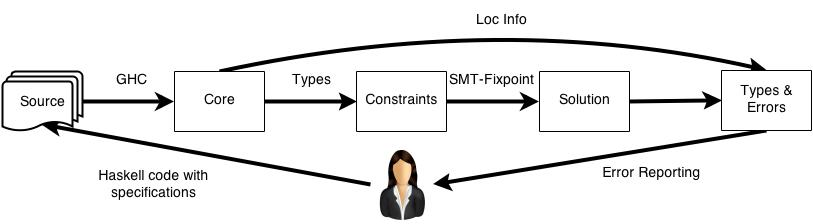
\includegraphics[width=\textwidth]{text/realworldhaskell/liquidHaskell}}
\caption{\toolname Workflow}
	\label{fig:internals}
\end{figure*}
% 
% link for workflow
% https://www.draw.io/#G0Bwp_mIorSVqJb2RENnNVWVlQTmc
%
We will start with a short description of the \toolname workflow,
summarized in Figure~\ref{fig:internals}, and continue with an 
example driven overview of how properties are specified
and verified using the tool. 

% \mypara{Usage} 
\mypara{Source}
\toolname can be run from the command-line\footnote{\url{https://hackage.haskell.org/package/liquidhaskell}}
or within a web-browser\footnote{\url{http://goto.ucsd.edu/liquid/haskell/demo/}}.
It takes as \emph{input}:
%
(1)~a single Haskell \emph{source} file with code and refinement
    type specifications including refined datatype definitions, 
    measures (\S~\ref{sec:tool:measures}), predicate and type 
    aliases, and function signatures;
%
(2)~a set of directories containing \emph{imported modules} 
    (including the \verb+Prelude+) which may themselves 
    contain specifications for exported types and functions; and
%
(3)~a set of predicate fragments called \emph{qualifiers},
    which are used to infer refinement types. This set is 
    typically empty as the default set of qualifiers extracted 
    from the type specifications suffices for inference.

\mypara{Core}
\toolname uses GHC to reduce the source to the Core IL~\cite{SulzmannCJD07}, 
and, to facilitate source-level error reporting, creates a map from Core 
expressions to locations in the Haskell source.

\mypara{Constraints}
Then, it uses the abstract interpretation framework of Liquid Typing~\cite{LiquidPLDI08}, 
modified to ensure soundness under lazy evaluation~\citep{LiquidICFP14},
to generate logical constraints from the Core IL.
     
\mypara{Solution}
Next, it uses a fixpoint algorithm (from~\citep{LiquidPLDI08})
combined with an SMT solver to solve the constraints, and hence 
infers a valid refinement typing for the program. 
%
\toolname can use any solver that implements the SMT-LIB2
standard~\cite{SMTLIB2}, including Z3~\citep{Z3}, CVC4~\citep{CVC4}, and
MathSat~\citep{MathSat}.

 
\mypara{Types \& Errors}
% \NV{satisfiability and validity refer to different things here, 
% which is confusing...}
If the set of constraints is satisfiable, then \toolname outputs 
\textsc{Safe}, meaning the program is verified.
If instead, the set of constraints is not satisfiable, then \toolname
outputs \textsc{Unsafe}, and uses the invalid constraints to 
report refinement type errors at the \emph{source positions}
that created the invalid constraints, using the location 
information to map the invalid constraints to source positions.
%
In either case, \toolname produces as output a source map
containing the \emph{inferred} types for each program 
expression, which, in our experience, is crucial for 
debugging the code and the specifications.

%\mypara{Optional Typing}
%
\toolname is best thought of as an \emph{optional} type checker
for Haskell. By optional we mean that the refinements have \emph{no} 
influence on the dynamic semantics, which makes it easy to apply 
\toolname to \emph{existing} libraries.
%
To emphasize the optional nature of refinements and preserve 
compatibility with existing compilers, all specifications 
appear within comments of the form \verb|{-@ ... @-}|, 
which we omit below for brevity.

\subsection{Specifications}

A refinement type is a Haskell type where each component
of the type is decorated with a predicate from a (decidable)
refinement logic. We use the quantifier-free logic of equality, 
uninterpreted functions and linear arithmetic (QF-EUFLIA)~\cite{Nelson81}. 
For example,
%
\begin{code}
   {v:Int | 0 <= v && v < 100}
\end{code}
%
describes @Int@ values between @0@ and @100@.

\mypara{Type Aliases} For brevity and readability, it is often convenient 
to define abbreviations for particular refinement predicates and types.
For example, we can define an alias for the above predicate
%
\begin{code}
  predicate Btwn Lo N Hi = Lo <= N && N < Hi
\end{code}
%
and use it to define a \emph{type alias}
%
\begin{code}
  type Rng Lo Hi = {v:Int | (Btwn Lo v Hi)} 
\end{code}
%
We can now describe the above integers as @(Rng 0 100)@.

\mypara{Contracts} 
To describe the desired properties of a function, we need
simply refine the input and output types with predicates 
that respectively capture suitable pre- and post-conditions. 
For example,
%
\begin{code}
  range :: lo:Int -> hi:{Int | lo <= hi} 
        -> [(Rng lo hi)]
\end{code}
%
states that @range@ is a function that takes two @Int@s 
respectively named @lo@ and @hi@ and returns a list of @Int@s 
between @lo@ and @hi@. There are three things worth
noting.
%
First, we have binders to name the function's \emph{inputs} 
(\eg, @lo@ and @hi@) and can use the binders inside the 
function's \emph{output}.
%
Second, the refinement in the \emph{input} type describes the 
\emph{pre-condition} that the second parameter @hi@ cannot 
be smaller than the first @lo@.
%
Third, the refinement in the \emph{output} type describes the
\emph{post-condition} that all returned elements are between 
the bounds of @lo@ and @hi@.


\subsection{Verification}\label{sec:tool:verification}

Next, consider the following implementation for @range@:
%
\begin{code}
  range lo hi 
    | lo <= hi  = lo : range (lo + 1) hi
    | otherwise = []
\end{code}
%
When we run \toolname on the above code, it reports an 
error at the definition of @range@. This is unpleasant! 
One way to debug the error is to determine what type has
been \emph{inferred} for @range@, \eg, by hovering the 
mouse over the identifier in the web interface. 
In this case, we see that the output type is essentially:
%
\begin{code}
  [{v:Int | lo <= v && v <= hi}]
\end{code}
%
which indicates the problem. There is an \emph{off-by-one} 
error due to the problematic guard. If we replace the second @<=@ 
with a @<@ and re-run the checker, the function is verified.

\mypara{Holes} It is often cumbersome to specify the Haskell
types, as those can be gleaned from the regular type signatures 
or via GHC's inference. Thus, \toolname allows the user to leave 
holes in the specifications. Suppose @rangeFind@ has type 
%
\begin{code}
  (Int -> Bool) -> Int -> Int -> Maybe Int
\end{code}
%
where the second and third parameters define a range. 
We can give @rangeFind@ a refined specification:
%
\begin{code}
  _ -> lo:_ -> hi:{Int | lo <= hi} 
    -> Maybe (Rng lo hi)
\end{code}
%
where the @_@ is simply the unrefined Haskell type for the 
corresponding position in the type.

\mypara{Inference} Next, consider the implementation
%
\begin{code}
  rangeFind f lo hi = find f $ range lo hi 
\end{code}
%$
where @find@ from @Data.List@ has the (unrefined) type
%
\begin{code}
  find :: (a -> Bool) -> [a] -> Maybe a
\end{code}
%
\toolname uses the abstract interpretation framework of 
Liquid Typing~\cite{LiquidPLDI08} to infer that the type
parameter @a@ of @find@ can be instantiated with @(Rng lo hi)@
thereby enabling the automatic verification of @rangeFind@.

Inference is crucial for automatically synthesizing types
for polymorphic instantiation sites -- note there is another
instantiation required at the use of the apply operator 
@$@ --  and to relieve the programmer of the tedium of %$
specifying signatures for all functions. 
%
Of course, for functions exported by the module,
we must write signatures to specify preconditions -- otherwise, 
the system defaults to using the trivial (unrefined) Haskell 
type as the signature \ie, checks the implementation assuming 
arbitrary inputs.

\subsection{Measures}\label{sec:tool:measures}
%% \NV{DONE(R1)
%% measure is introduced as something that gives the size of a value, 
%% but it is later used for more general properties e.g. almostRB 
%% over red-black trees.
%% }
So far, the specifications have been limited to comparisons and 
arithmetic operations on primitive values. 
We use \emph{measure functions}, or just measures, to 
specify \emph{inductive properties} of algebraic data types. 
%
For example, we define a measure @len@ to write properties about the number
of elements in a list.
%
\begin{code}
  measure len :: [a] -> Int
  len []      = 0
  len (x:xs)  = 1 + (len xs)
\end{code}
%
Measure definitions are \emph{not} arbitrary Haskell code but a very 
restricted subset~\cite{LiquidICFP14}.
Each measure has a single equation per constructor that defines the
value of the measure for that constructor. The right-hand side of the 
equation is a term in the restricted refinement logic. Measures are 
interpreted by generating refinement types for the corresponding 
data constructors.
%
For example, from the above, \toolname derives the 
following types for the list data constructors:
%
\begin{code}
  []  :: {v:[a]| len v = 0}
  (:) :: _ -> xs:_ -> {v:[a]| len v = 1 + len xs}
\end{code}
%
Here, @len@ is an \emph{uninterpreted function} in the refinement logic.
We can define multiple measures for a type; \toolname simply conjoins
the individual refinements arising from each measure to obtain a single
refined signature for each data constructor.

\mypara{Using Measures}
We use measures to write specifications about algebraic types. 
For example, we can specify and verify that: 
%
\begin{code}
  append :: xs:[a] -> ys:[a] 
         -> {v:[a]| len v = len xs + len ys}

  map    :: (a -> b) -> xs:[a] 
         -> {v:[b]| len v = len xs} 

  filter :: (a -> Bool) -> xs:[a] 
         -> {v:[a]| len v <= len xs}
\end{code}

\mypara{Propositions} 
%%In addition to allowing the specification of structural features like
%%lengths, heights and so on, 
Measures can be used to encode sophisticated 
invariants about algebraic data types.
%
To this end, the user can write a measure whose output has a special type 
@Prop@ denoting propositions in the refinement logic. For instance, we can
describe a list that contains a @0@ as:
%
\begin{code}
  measure hasZero :: [Int] -> Prop
  hasZero []      = false
  hasZero (x:xs)  = x == 0 || (hasZero xs) 
\end{code}
%
We can then define lists containing a @0@ as:
%
\begin{code}
  type HasZero = {v : [Int] | (hasZero v)} 
\end{code}
%
Using the above, \toolname will accept 
%
\begin{code}
  xs0 :: HasZero 
  xs0 = [2,1,0,-1,-2]
\end{code}
%
but will reject
%
\begin{code}
  xs' :: HasZero 
  xs' = [3,2,1]
\end{code}



\subsection{Refined Data Types}

Often, we require that \emph{every} instance of a type satisfies some invariants. 
For example, consider a @CSV@ data type, that represents tables:
%
\begin{code}
  data CSV a = CSV { cols :: [String]
                   , rows :: [[a]]    }
\end{code}
%
% With \toolname we can enforce the invariant that for every @CSV@ table, 
% with a number of columns given by @dim@,
% each row has @dim@ elements,
% with the below refined data type definition
%%With \toolname we can enforce the invariant that every @CSV@ table 
%%has the number of columns given by @dim@, and that each row has 
%%@dim@ elements with a refined data type definition, such as:
With \toolname we can enforce the invariant that every row in a @CSV@ table
should have the same number of columns as there are in the header
%
\begin{code}
  data CSV a = CSV { cols :: [String]  
                   , rows :: [ListL a cols] }
\end{code}
%
using the alias
%
\begin{code}
  type ListL a X = {v:[a]| len v = len X}
\end{code}
%
A refined data definition is \emph{global} in that \toolname 
will reject any @CSV@-typed expression that does not respect 
the refined definition. For example, both of the below 
%
\begin{code}
  goodCSV = CSV [  "Month", "Days"] 
                [ ["Jan"  , "31"]
                , ["Feb   , "28"]
                , ["Mar"  , "31"] ]

  badCSV  = CSV [  "Month", "Days"] 
                [ ["Jan"  , "31"]
                , ["Feb   , "28"]
                , ["Mar"        ] ]
\end{code}
%
are well-typed Haskell, but the latter is rejected by \toolname.
%
Like measures, the global invariants are enforced by refining 
the constructors' types. 

\subsection{Refined Type Classes}\label{sec:type-classes}

Next, let us see how \toolname supports the verification of
programs that use ad-hoc polymorphism via type classes.
%
While the implementation of each typeclass instance is 
different, there is often a common interface that we 
expect all instances to satisfy.

\mypara{Class Measures}
As an example, consider the class definition
%
\begin{code}
  class Indexable f where
    size :: f a -> Int
    at   :: f a -> Int -> a
\end{code}
%
For safe access, we might require that @at@'s second 
parameter is bounded by the @size@ of the container.
To this end, we define a \emph{type-indexed} 
measure, using the @class measure@ keyword
%
\begin{code}
  class measure sz :: a -> Nat
\end{code}
%
Now, we can specify the safe-access precondition  
independent of the particular instances of @Indexable@:
%
\begin{code}
  class Indexable f where
    size :: xs:_ -> {v:Nat | v = sz xs}
    at   :: xs:_ -> {v:Nat | v < sz xs} -> a
\end{code}

\mypara{Instance Measures}
For each concrete type that instantiates a class, we require 
a corresponding definition for the measure. 
For example, to define lists as an instance of @Indexable@, 
we require the definition of the @sz@ instance for lists:
%
\begin{code}
  instance measure sz :: [a] -> Nat
  sz []     = 0
  sz (x:xs) = 1 + (sz xs)
\end{code}
%
Class measures work just like regular measures in that the above 
definition is used to refine the types of the list data constructors.
After defining the measure, we can define the type instance as:
%
\begin{code}
  instance Indexable [] where
    size []        = 0
    size (x:xs)    = 1 + size xs

    (x:xs) `at` 0  = x
    (x:xs) `at` i  = index xs (i-1)
\end{code}
%
\toolname uses the definition of @sz@ for lists to check that @size@ 
and @at@ satisfy the refined class specifications. 
% NV the dictionary relevant this were removed
% , and hence, that 
% the above creates a valid instance dictionary for @Indexable@.

\mypara{Client Verification}
At the clients of a type-class we use the refined 
types of class methods. Consider a client of @Indexable@s:
%
\begin{code}
  sum :: (Indexable f) => f Int -> Int
  sum xs = go 0 
    where
      go i | i < size xs = xs `at` i + go (i+1)
           | otherwise   = 0
\end{code}
%
\toolname proves that each call to @at@ is safe, by using the refined
class specifications of @Indexable@. 
Specifically, each call to @at@ is guarded by a check @i < size xs@
and @i@ is  increasing 
from 0, so \toolname proves that @xs `at` i@ will always be safe.

\subsection{Abstracting Refinements}

So far, all the specifications have used \emph{concrete} refinements. Often it is
useful to be able to \emph{abstract} the refinements that appear in a
specification. For example, consider a monomorphic variant of @max@
%
\begin{code}
  max     :: Int -> Int -> Int 
  max x y = if x > y then x else y
\end{code}
%
We would like to give @max@ a specification that lets us verify:
%
\begin{code}
  xPos  :: {v: _ | v > 0}
  xPos  = max 10 13

  xNeg  :: {v: _ | v < 0}
  xNeg  = max (-5) (-8)

  xEven :: {v: _ | v mod 2 == 0} 
  xEven = max 4 (-6)
\end{code}
%
To this end, \toolname allows the user to \emph{abstract refinements} over
types~\cite{vazou13}, for example by typing @max@ as:
%
\begin{code}
 max :: forall <p :: Int -> Prop>. 
          Int<p> -> Int<p> -> Int<p>
\end{code}
%
The above signature states that for any refinement @p@, if the two
inputs of @max@ satisfy @p@ then so does the output. \toolname uses
Liquid Typing to automatically instantiate @p@ with suitable concrete
refinements, thereby checking @xPos@, @xNeg@, and @xEven@.


\mypara{Dependent Composition}
Abstract refinements turn out to be a surprisingly expressive and 
useful specification mechanism. For example, consider the function 
composition operator:
%
\begin{code}
  (.) :: (b -> c) -> (a -> b) -> a -> c
  (.) f g x = f (g x)  
\end{code}
%
Previously, it was not possible to check, \eg that:
%
\begin{code}
  plus3 :: x:_ -> {v:_ | v = x + 3}
  plus3 = (+ 1) . (+ 2)
\end{code}
%
as the above required tracking the dependency between @a@, @b@ and @c@,
which is crucial for analyzing idiomatic Haskell.
With abstract refinements, we can give the @(.)@ operator the type:
%
\begin{code}
  (.) :: forall < p :: b -> c -> Prop
                , q :: a -> b -> Prop>.
           f:(x:b -> c<p x>) 
        -> g:(x:a -> b<q x>) 
        -> y:a 
        -> exists[z:b<q y>].c<p z>
\end{code}
%
which gets automatically instantiated at usage sites, allowing \toolname
to precisely track invariants through the use of the ubiquitous 
higher-order operator.

\mypara{Dependent Pairs}
Similarly, we can abstract refinements over the definition of datatypes.
% Similarly, we can abstract refinements over the definition of datatypes.
For example, we can express dependent pairs in \toolname by refining the 
definition of tuples as:
%
\begin{code}
  data Pair a b <p :: a -> b -> Prop> 
    = Pair { fst :: a, snd :: b<p fst>}
\end{code}
%
That is, the refinement @p@ relates the @snd@ element with the @fst@.
Now we can define increasing and decreasing pairs
%
\begin{code}
  type IncP = Pair <{\x y -> x < y}> Int Int
  type DecP = Pair <{\x y -> x > y}> Int Int
\end{code}
%
and then verify that:
%
\begin{code}
  up :: IncP
  up = Pair 2 5
  
  dn :: DecP
  dn = Pair 5 2
\end{code}
%
Now that we have a bird's eye view of the various specification mechanisms
supported by \toolname, let us see how we can profitably apply them to
statically check a variety of correctness properties in real-world codes.

%%% Local Variables: 
%%% mode: latex
%%% TeX-master: "main"
%%% End: 

\section{Totality}\label{sec:totality}
%% OK \NV{DONE intro (R1)
%% OK Sections 3 and 4 cover "totality" and "termination" respectively. It would be helpful to explain these terms at the start of section 3, so that the two are distinguished appropriately.
%% OK }
Well typed Haskell code can go very wrong:
%
\begin{code}
  *** Exception: Prelude.head: empty list
\end{code}
%
As our first application, let us see how to use 
\toolname to statically guarantee the absence
of such exceptions, \ie, to prove various 
functions \emph{total}.

\subsection{Specifying Totality}

First, let us see how to specify the notion of
totality inside \toolname. Consider the source of 
the above exception:
%
\begin{code}
  head :: [a] -> a
  head (x:_) = x
\end{code}
%
Most of the work towards totality checking is done by 
the translation to GHC's Core, in which every function 
\emph{is} total, but may explicitly call an \emph{error} 
function that takes as input a string that describes the 
source of the pattern-match failure and throws an exception.
%
For example @head@ is translated into
%
\begin{code}
  head d = case d of 
             x:xs -> x
             []   -> patError "head"
\end{code}

Since every core function is total, but may explicitly 
call error functions, to prove that the source function is 
total, it suffices to prove that @patError@ 
will \emph{never} be called.
%
We can specify this requirement by giving the error 
functions a @false@ pre-condition:
%
\begin{code}
  patError :: {v:String | False } -> a
\end{code}
%
The pre-condition states that the input type is \emph{uninhabited}
and so an expression containing a call to @patError@ will only type 
check if the call is \emph{dead code}.


\subsection{Verifying Totality}

The (core) definition of @head@ does not typecheck
as is; but requires a pre-condition that states that the function
is only called with non-empty lists. Formally, we do so by 
defining the alias
%
\begin{code}
  predicate NonEmp X = 0 < len X 
\end{code}
%
and then stipulating that 
%
\begin{code}
  head :: {v : [a] | NonEmp v} -> a
\end{code}
%
To verify the (core) definition of @head@, \toolname uses the above signature
to check the body in an environment
%
\begin{code}
  d :: {0 < len d}
\end{code}
%
When @d@ is matched with @[]@, the environment is 
strengthened with the corresponding refinement from 
the definition of @len@, \ie,
%
\begin{code}
  d :: {0 < (len d) && (len d) = 0}
\end{code}
%
Since the formula above is a contradiction, \toolname concludes that the
call to @patError@ is dead code, and thereby verifies the totality 
of @head@. Of course, now we have pushed the burden of proof onto clients
of @head@ -- at each such site, \toolname will check that the argument 
passed in is indeed a @NonEmp@ list, and if it successfully does so, then
we, at any uses of @head@, can rest assured that @head@ will never throw an 
exception. 

\mypara{Refinements and Totality} 
While the @head@ example is quite simple, in general, refinements make
it easy to prove totality in complex situations, where we must track
dependencies between inputs and outputs. For example, consider the @risers@
function from \cite{catch}:
%
\begin{code}
  risers []       = []
  risers [x]      = [[x]]
  risers (x:y:zs) 
    | x <= y      = (x:s) : ss 
    | otherwise   = [x] : (s:ss) 
    where 
      s:ss    = risers (y:etc)
\end{code}
%
The pattern match on the last line is partial; its core translation is
%
\begin{code}
  let (s, ss) = case risers (y:etc) of
                  s:ss -> (s, ss)
                  []   -> patError "..."
\end{code}
%
What if @risers@ returns an empty list? 
Indeed, @risers@ \emph{does}, on occasion, return an empty list per its
first equation. However, on close inspection, it turns out that 
\emph{if} the input is non-empty, \emph{then} the output is also
non-empty. Happily, we can specify this as:
%
\begin{code}
  risers :: l:_ -> {v:_ | NonEmp l => NonEmp v} 
\end{code}

\toolname verifies that @risers@ meets the above specification, 
and hence that the @patError@ is dead code as at that 
site, the scrutinee is obtained from calling @risers@ with a
@NonEmp@ list.

\mypara{Non-Emptiness via Measures}
Instead of describing non-emptiness indirectly using @len@, a 
user could a special measure:
%
\begin{code}
  measure nonEmp  :: [a] -> Prop
  nonEmp (x:xs)   = True
  nonEmp []       = False

  predicate NonEmp X = nonEmp X
\end{code}
%
After which, verification would proceed analagous to the above.

\mypara{Total Totality Checking} 
@patError@ is one of many possible errors thrown by non-total functions.  
@Control.Exception.Base@ has several others including @recSelError@, @irrefutPatError@, \etc which serve the purpose of making 
core translations total.
%
Rather than hunt down and specify @False@ preconditions one
by one, the user may automatically turn on totality checking 
by invoking \toolname with the \cmdtotality command line option, 
at which point the tool systematically checks that all the above 
functions are indeed dead code, and hence, that all definitions are total.

\subsection{Case Studies}

We verified totality of two libraries: \lbhscolour and \lbmap, earlier versions
of which had previously been proven total by \texttt{catch}~\citep{catch}.

\mypara{\lbmap} 
is a widely used library for (immutable) key-value maps, implemented
as balanced binary search trees.
Totality verification of \lbmap was quite straightforward.
We had already verified termination and the crucial 
binary search invariant~\ref{chapter:abstractrefinements}. To verify 
totality it sufficed to simply re-run verification with
the \cmdtotality argument.
%
All the important specifications were already captured by the types, 
and no additional changes were needed to prove totality.
%
%% \RJ{was it trivially total? i.e. is it total if you strip out all refinements
%% from specs?}
%% \NV{No, it fails in 6 functions all of which can trivially be reasoned to be total}
%% \NV{hedgeUnion, hedgeDiff, hedgeMerge, submap', join, merge}
%% \NV{The interesting story is that during verification \emph{we accidentally modified}
%% turn a function to partial, see my commit 041f1f0fea4d34ee41f50dbf7ce43e3c084c2743}
%

This case study illustrates an advantage of \toolname over specialized provers 
(\eg, \texttt{catch}~\citep{catch}): it can be used to prove totality, termination and
functional correctness at the same time, facilitating a nice reuse of
specifications for multiple tasks.

%% DONE \NV{(R3)
%% DONE Before discussing HsColour, I'd give a brief explanation of what it is.
%% DONE }
\mypara{\lbhscolour} is a library for generating syntax-highlighted LATEX and HTML from
Haskell source files.
Checking \lbhscolour was not so easy, as in some cases assumptions are used about the 
structure of the input data:
%
For example, @ACSS.splitSrcAndAnnos@ handles an
input list of @String@s and assumes that whenever
a specific @String@ (say @breakS@) appears then 
at least two @String@s (call them @mname@ and @annots@)
follow it in the list.
Thus, for a list @ls@ that starts with @breakS@ 
the irrefutable pattern  @(_:mname:annots)@ @=@ @ls@
should be total.
%
Though possible, it is currently it is somewhat cumbersome to specify such 
properties. 
%
As an easy and practical solution, 
to prove totality, we added a dynamic check that 
validates that the length of the input @ls@ exceeds @2@.

%% measure follows a b c = \case 
%%   []   -> true
%%   x:xs -> if x == a then first2 b c xs else follows a b c xs
%% 
%% measure first2 b c = \case
%%   []   -> false
%%   x:xs -> x == b && first1 c xs
%% 
%% measure first1 c = \case
%%   []   -> false
%%   x:xs -> x == c
%% 
%% Worse, \toolname has no way to express such an invariant: 
%% \toolname naturally describes invariants that recursively 
%% hold for every list element and 
%% reaches its limitations when reasoning about non-recursive
%% properties.

In other cases assertions were imposed via monadic checks, \eg @HsColour.hs@ reads the input arguments and 
checks their well-formedness using 
%
\begin{code}
  when (length f > 1) $ errorOut "..."
\end{code} %$
%
Currently \toolname does not support monadic reasoning that 
allows assuming that @(length f <= 1)@
holds when executing the action \emph{following} the @when@ check. 
%
Finally, code modifications were required to capture properties 
that are cumbersome to express with \toolname.
%
For example, @trimContext@ checks if there is an element that 
satisfies @p@ in the list @xs@; if so it defines 
%
@ys = dropWhile (not . p) xs@
%
and computes @tail ys@.
%
By the check we know that @ys@ has at least one element, the 
one that satisfies @p@. 
%
Due to the complexity of this property, we preferred to rewrite the specific code 
in a more verification friendly version. 


%%% \mynote{Bug}
%%% %
%%% \RJ{WHY? Seems like a simple GHC CHECK?}
%%% %
%%% On the positive side, totality verification revealed a subtle bug:
%%% %
%%% The instance @Enum@ of @Highlight@ does not define the @toEnum@ 
%%% method. In core, this reduces to a call to the error function 
%%% @noMethodBinding@.
%%% %
%%% Even though this totality bug can be tracked by GHC compilation,
%%% it exposes the strengths of our totality checker.

On the whole, while proving totality can be cumbersome 
(as in \lbhscolour) it is a nice side benefit of refinement
type checking and can sometimes be a fully automatic corollary
of establishing more interesting safety properties (as in \lbmap).

\section{Termination}\label{sec:termination}

To soundly account for Haskell's non-strict evaluation, a refinement
type checker must distinguish between terms that may potentially 
diverge and those that will not~\cite{LiquidICFP14}.
%
Thus, by default, \toolname proves termination of each recursive function.
Fortunately, refinements make this onerous task quite straightforward. 
We need simply associate a \emph{well-founded termination metric} % $\mu$
on the function's parameters, and then use refinement typing to check 
that the metric strictly decreases at each recursive call. In practice,
due to a careful choice of defaults, this amounts to about a line 
of termination-related hints per hundred lines of source. 
Details about the termination checker may be found in \cite{LiquidICFP14}, 
we include a brief description here to make the paper self-contained.

\mypara{Simple Metrics}
As a starting example, consider the @fac@ function
%
\begin{code}
  fac :: n:Nat -> Nat / [n]
  fac 0 = 1 
  fac n = n * fac (n-1)
\end{code}
%
The termination metric is simply the parameter @n@; 
as @n@ is non-negative and decreases at the recursive 
call, \toolname verifies that @fac@ will terminate.
%
We specify the termination metric in the type signature 
with the @/[n]@.

Termination checking is performed at the same 
time as regular type checking, as it can be 
reduced to refinement type checking with a 
special terminating fixpoint combinator~\cite{LiquidICFP14}.
Thus, if \toolname fails to prove that a given 
termination metric is well-formed and decreasing, 
it will report a @Termination Check@ @Error@. 
%% \RJ{Seems untrue -- I just get a plain old liquid type error?
%% NV: IF you provide termination metrics, you DO get termination check error}.
At this point, the user can either debug 
the specification, or mark the function 
as non-terminating.


%%\mypara{Refinements Enable Termination} 
%%Consider Euclid's GCD:
%%%
%%\begin{code}
%%  gcd :: a:Nat -> {v:Nat | v < a} -> Nat 
%%  gcd a 0 = a
%%  gcd a b = gcd b (a `mod` b)
%%\end{code}
%%%
%%Here, the termination metric is the first parameter @a@.
%%To prove that @a@ is decreasing requires
%%the fact that the second parameter is smaller than the first 
%%and that @mod@ returns results smaller than its second 
%%parameter. Both facts are easily expressed as refinements, 
%%but elude non-extensible checkers~\cite{Giesl11}.
%%
%%\mypara{Explicit Termination Metrics}
%%The termination metric can be some parameter \emph{other} than the first 
%%argument.
%%For example, consider: % As an example, consider the tail-recursive factorial:
%%%
%%\begin{code}
%%  tfac     :: Nat -> n:Nat -> Nat / [n] 
%%  tfac x 0 = if n == 0 then x
%%                       else tfac (n*x) (n-1)
%%\end{code}
%%%
%%%
%%It can be checked that @n@, \ie, the second argument is decreasing at each recursive call.
%%
\mypara{Termination Expressions} 
Sometimes, no single parameter decreases across recursive calls,
but there is some \emph{expression} that forms the decreasing 
metric.
%
For example recall @range lo hi@ (from \S~\ref{sec:tool:verification}) 
which returns the list of @Int@s from @lo@ to @hi@:
%
\begin{code}
  range lo hi 
    | lo < hi   = lo : range (lo+1) hi
    | otherwise = [] 
\end{code}
%
Here, neither parameter is decreasing (indeed, the first 
one is increasing) but @hi-lo@ decreases across each call. 
To account for such cases, we can specify as the termination
metric a (refinement logic) expression over the function
parameters. Thus, to prove termination, we could type @range@ as:
\begin{code}
  lo:Int -> hi:Int -> [(Btwn lo hi)] / [hi-lo]
\end{code}

\mypara{Lexicographic Termination}
The Ackermann function
%
\begin{code}
  ack m n 
    | m == 0    = n + 1
    | n == 0    = ack (m-1) 1 
    | otherwise = ack (m-1) (ack m (n-1))
\end{code}
%
is curious as there exists no simple, natural-valued, 
termination metric that decreases at each recursive call.
%
However @ack@ terminates because at each call \emph{either}
@m@ decreases \emph{or} @m@ remains the same and @n@ decreases. 
%
In other words, the pair @(m,n)@ strictly decreases according to a
\emph{lexicographic} ordering. 
%
Thus \toolname supports termination metrics that are a 
\emph{sequence of} termination expressions. For example, 
we can type @ack@ as:
%
\begin{code}
  ack :: m:Nat -> n:Nat -> Nat / [m, n]
\end{code}
%
At each recursive call \toolname uses a lexicographic 
ordering to check that the sequence of termination 
expressions is decreasing (and well-founded in each component).

\mypara{Mutual Recursion}
%
The lexicographic mechanism lets us check termination of
mutually recursive functions, \eg @isEven@ and @isOdd@
%
\begin{code}
  isEven 0 = True
  isEven n = isOdd $ n-1
  
  isOdd n  = not $ isEven n 
\end{code}
%
Each call terminates as either @isEven@ calls @isOdd@ with a 
decreasing parameter, \emph{or} @isOdd@ calls @isEven@ with 
the same parameter, expecting the latter to do the decreasing.
%
For termination, we type:
%
\begin{code}
  isEven :: n:Nat -> Bool / [n, 0]
  isOdd  :: n:Nat -> Bool / [n, 1]
\end{code}
%
To check termination, \toolname verifies that at each recursive 
call the metric of the caller is less than the metric of the 
callee.
%
When @isEven@ calls @isOdd@, it proves that the caller's 
metric, namely @[n,0]@ is greater than the callee's @[n-1,1]@.
When \hbox{@isOdd@} calls @isEven@, it proves that the 
caller's metric @[n,1]@ is greater than the callee's @[n,0]@,
thereby proving the mutual recursion always terminates.

\mypara{Recursion over Data Types}
The above strategies generalize easily to functions that recurse
over (finite) data structures like arrays, lists, and trees.
In these cases, we simply use \emph{measures} to project the 
structure onto @Nat@, thereby reducing the verification to 
the previously seen cases. 
For example, we can prove that @map@ 
%
\begin{code}
  map f (x:xs) = f x : map f xs
  map f []     = []
\end{code}
%
terminates, by typing @map@ as 
%
\begin{code}
  (a -> b) -> xs:[a] -> [b] / [len xs]
\end{code}
%
\ie, by using the measure @len xs@, from \S~\ref{sec:tool:measures}, 
as the metric.

%%% %
%%% \begin{code}
%%%   data L [sz] a = N | C a (L a)
%%% \end{code}
%%% %
%%% we can define a \emph{measure}
%%% %
%%% \begin{code}
%%%   measure sz  :: L a -> Nat
%%%   sz (C x xs) = 1 + (sz xs)
%%%   sz N        = 0
%%% \end{code}
%%% %
%%% We prove that @map@ terminates using the type:
%%% %
%%% \begin{code}
%%%   map :: (a -> b) -> xs:L a -> L b / [sz xs]
%%%   map f (C x xs) = C (f x) (map f xs)
%%%   map f N        = N
%%% \end{code}
%%% %
%%% That is, by simply using @(sz xs)@  as the 
%%% decreasing metric.

\mypara{Generalized Metrics Over Datatypes}
In many functions there is no single argument 
whose measure provably decreases. Consider
%
\begin{code}
  merge (x:xs) (y:ys)
    | x < y     = x : merge xs (y:ys)
    | otherwise = y : merge (x:xs) ys
\end{code}
%
from the homonymous sorting routine. Here, neither
parameter decreases, but the \emph{sum} of their 
sizes does. To prove termination, we can type @merge@ as:
%
\begin{code}
  xs:[a] -> ys:[a] -> [a] / [len xs + len ys]
\end{code}

%%%% \begin{figure*}[!t]
%%%% 	\begin{code}
%%%% 	type OL  a   =  [a]<{\fld v -> (v >= fld)}>
%%%% 
%%%% 	qsort :: (Ord a) => xs:[a] -> OL a / [(len xs), 0]
%%%% 	qsort []         = []
%%%% 	qsort (x:xs)     = qpart x xs [] []
%%%% 
%%%% 	qpart :: (Ord a) => x:a -> q:[a] -> r: [{v:a|v<x}] -> p: [{v:a|v>=x}] -> OL a 
%%%% 	       / [((len q) + (len r) + (len p)), ((len q) + 1)]
%%%% 	qpart x []     rlt rge             = app x (qsort rlt) (x:qsort rge)
%%%% 	qpart x (y:ys) rlt rge | x > y     = qpart x ys (y:rlt) rge
%%%% 	                       | otherwise = qpart x ys rlt (y:rge)
%%%% 
%%%% 	app k []     ys = ys
%%%% 	app k (x:xs) ys = x : (app k xs ys)
%%%% 	\end{code}
%%%% \caption{Mutual-recursive qsort}
%%%% \label{fig:code:qsort}
%%%% \end{figure*}


\mypara{Putting it all Together}
The above techniques can be combined to prove 
termination of the mutually recursive quick-sort (from~\citep{XiTerminationLICS01})% \RJ{from where?}
%
\begin{code}
  qsort (x:xs)   = qpart x xs [] []
  qsort []       = []

  qpart x (y:ys) l r 
    | x > y      = qpart x ys (y:l) r 
    | otherwise  = qpart x ys l (y:r)
  qpart x [] l r = app x (qsort l) (qsort r) 

  app k []     z = k : z
  app k (x:xs) z = x : app k xs z
\end{code}
%
@qsort (x:xs)@ calls @qpart x xs@ to partition @xs@ 
into two lists @l@ and @r@ that have elements less 
and greater or equal than the pivot @x@, respectively.
%
When @qpart@ finishes partitioning it mutually recursively
calls @qsort@ to sort the two list and appends the results 
with @app@. 
%
\toolname proves sortedness as well~\cite{vazou13} but let us 
focus here on termination. To this end, we type the functions
as:
%
\begin{code}
  qsort :: xs:_ -> _ 
        / [len xs, 0]
    
  qpart :: _ -> ys:_ -> l:_ -> r:_ -> _ 
        / [len ys + len l + len r, 1 + len ys]
\end{code}
%
As before, \toolname checks that at each recursive call 
the caller's metric is less than the callee's. 
%
When @qsort@ calls @qpart@ the length of the unsorted 
list @len (x:xs)@ exceeds the \hbox{@len xs + len [] + len []@}.
%
When @qpart@ recursively calls itself the first component
of the metric is the same, but the length of the unpartitioned 
list decreases, \ie @1 + len y:ys@ exceeds \hbox{@1 + len ys@}.
%
Finally, when @qpart@ calls @qsort@ we have \hbox{@len ys + len l + len r@}
exceeds both @len l@ and @len r@, thereby ensuring termination.


%%% Before we dive into proving termination, note that the 
%%% type alias @OL a@ uses Abstract Refinements~\citep{vazou13} to describe 
%%% Ordered Lists. 
%%% Thus, when \toolname decides that the @qsort@ is SAFE, 
%%% it proves both termination and sortedness.
%%%%Note that classical appending @rlt ++ rge@ of the two sorted lists will lose 
%%%%the crucial for sorting information that every element of @rlt@ is less than each element of @rge@.
%%%%%
%%%%Thus we defined a new version of list appending @app@ that uses the pivot element @k@
%%%%as a ghost-parameter.
%%%%%
%%%%Good news is that \toolname will automatically infer the appropriate type of @app@!

%% Let \mus{xs} and \mup{q}{r}{p} be the (well-founded) termination pairs
%% for @qsort xs@ and @qpart x q r p@ respectively, as annotated in the type signatures.
%% %
%%%$\mu_s(x:xs) = (1 + len xs, 0) > (len xs + 0 + 0, len xs + 1) = \mu_p(xs, [], [])$
%%%$\mu_p(y:ys, rlt, rge) = ((1 + (len ys)) + (len rlt) + (len rge), (1 + len ys) + 1) > 
%%%(len ys + (1 + (len rlt)) + (len rge), ((len ys) + 1)) = \mu_p(ys, y:rlt, rge) $
%%%$\mu_p([], rlt, rge) = (0 + len rlt + len rge, 1) > (len rlt, 0) = \mu_s(rlt)$ 

%% Existing techniques~\citep{CookPR11} could be used to 
%% come up with termination metrics.
%% We leave embedding these techniques into \toolname as a future work, and instead
%% we use some defaults to automate termination proving 
%% on functions with trivial metrics.

\mypara{Automation: Default Size Measures}
%
The @qsort@ example illustrates that while \toolname is 
very expressive, devising appropriate termination metrics 
can be tricky.
%
Fortunately, such patterns are very uncommon, and the vast
majority of cases in real world programs are just structural 
recursion on a datatype.
%
\toolname automates termination proofs for this common case,
by allowing users to specify a \emph{default size measure} 
for each data type, \eg @len@ for @[a]@.
%
Now, if no explicit termination metric is given, by default 
\toolname assumes that the \emph{first} argument whose type
has an associated size measure decreases.
%
Thus, in the above, we need not specify metrics for @fac@ 
or @map@ as the size measure is automatically 
used to prove termination. 
%
This heuristic suffices to \emph{automatically}
prove 67\% of recursive functions terminating.

\mypara{Disabling Termination Checking}
In \texttt{Haskell}'s lazy setting not all functions are terminating.
% 
\toolname provides two mechanisms the disable termination proving.
%
A user can disable checking a single function by marking 
that function as lazy. For example, specifying @lazy repeat@ 
tells the tool to not prove @repeat@ terminates.
%
Optionally, a user can disable termination checking for a whole
module by using the command line argument \cmdnotermination
for the entire file.

\section{Memory Safety}\label{sec:memory-safety}

The terms ``Haskell'' and ``pointer arithmetic'' rarely occur in the same
sentence, yet many Haskell programs are constantly manipulating pointers under
the hood by way of using the \bytestring and \libtext libraries. These libraries
sacrifice safety for (much needed) speed and are therefore natural candidates for
verification through \toolname.

\subsection{Bytestring}\label{sec:bytestring}
The single most important aspect of the \bytestring 
library, %~\cite{bytestring}, 
our first case study, is its pervasive intermingling of
high level abstractions like higher-order loops,
folds, and fusion, with low-level pointer 
manipulations in order to achieve high-performance. 
%
%% From the package description, \bytestring is, 
%% ``A time and space-efficient implementation of byte vectors using packed
%% Word8 arrays, suitable for high performance use, both in terms of large
%% data quantities, or high speed requirements. Byte vectors are encoded as
%% strict Word8 arrays of bytes, held in a ForeignPtr, and can be passed
%% between C and Haskell with little effort."
%
\bytestring is an appealing target for evaluating
\toolname, as refinement types are an ideal way to 
statically ensure the correctness of the delicate 
pointer manipulations, errors in which lie below 
the scope of dynamic protection.

The library spans $8$ files (modules) totaling about 3,500 lines.
We used \toolname to verify the library by giving precise 
types describing the sizes of internal pointers and bytestrings. 
These types are used in a modular fashion to verify the 
implementation of functional correctness properties of 
higher-level API functions which are built using 
lower-level internal operations. 
Next, we show the key invariants and how
\toolname reasons precisely about pointer
arithmetic and higher-order codes.

\spara{Key Invariants}
A (strict) @ByteString@ is a triple of a @pay@load pointer, 
an @off@set into the memory buffer referred to by the pointer 
(at which the string actually ``begins") and a @len@gth 
corresponding to the number of bytes in the string, which is 
the size of the buffer \emph{after} the @off@set, that
corresponds to the string.
%
We define a measure for the \emph{size} of 
a @ForeignPtr@'s buffer, and use it to define 
the key invariants as a refined datatype 
%
\begin{code}
  measure fplen  :: ForeignPtr a -> Int
  data ByteString = PS 
     { pay :: ForeignPtr Word8
     , off :: {v:Nat | v       <= fplen pay }
     , len :: {v:Nat | off + v <= fplen pay } }
\end{code}
%
The definition states that 
the offset is a @Nat@ no bigger than the size of 
the @payload@'s buffer, and that
the sum of the @off@set and non-negative @len@gth
is no more than the size of the payload buffer.
Finally, we encode a @ByteString@'s size as a measure.
%
\begin{code}
  measure bLen   :: ByteString -> Int
  bLen (PS p o l) = l
\end{code}

\spara{Specifications}
We define a type alias for a @ByteString@ whose length is the same
as that of another, and use the alias to type the API 
function @copy@, which clones @ByteString@s.

\begin{code}
  type ByteStringEq B = {v:ByteString | (bLen v) = (bLen B)}
  
  copy :: b:ByteString -> ByteStringEq b 
  copy (PS fp off len) 
    = unsafeCreate len $ \p -> 
        withForeignPtr fp $ \f ->
          memcpy len p (f `plusPtr` off) 
\end{code}

\spara{Pointer Arithmetic}
The simple body of @copy@ abstracts a fair bit of internal work. 
@memcpy sz dst src@, implemented in \C and accessed via the FFI is a potentially
dangerous, low-level operation, that copies @sz@ bytes starting
\emph{from} an address @src@ \emph{into} an address @dst@. 
Crucially, for safety, the regions referred to be @src@ and @dst@ 
must be larger than @sz@. We capture this requirement by defining
a type alias @PtrN a N@ denoting GHC pointers that refer to a region
bigger than @N@ bytes, and then specifying that the destination
and source buffers for @memcpy@ are large enough. 

\begin{code}
  type PtrN a N = {v:Ptr a | N <= (plen v)}
  memcpy :: sz:CSize -> dst:PtrN a siz 
                     -> src:PtrN a siz 
                     -> IO () 
\end{code}


The actual output for @copy@ is created and filled in using the 
internal function @unsafeCreate@ which is a wrapper around. 
% -- | Create ByteString of size @l@ and use
% --   action @f@ to fill it's contents.
\begin{code}
  create :: l:Nat -> f:(PtrN Word8 l -> IO ())
         -> IO (ByteStringN l)
  create l f = do
      fp <- mallocByteString l
      withForeignPtr fp $ \p -> f p
      return $! PS fp 0 l
\end{code}

% We include the comment to illustrate how the 
% refinement type captures the natural language 
% requirement in a machine checkable manner.
%
The type of @f@ specifies that the action
will only be invoked on a pointer of length at least 
@l@, which is verified by propagating the types of
@mallocByteString@ and @withForeignPtr@. 
%
The fact that the action is only invoked on such pointers 
is used to ensure that the value @p@ in the body of @copy@ 
is of size @l@. This, and the @ByteString@ 
invariant that the size of the payload @fp@ 
exceeds the sum of @off@ and @len@, ensures 
safety of the @memcpy@ call.

\spara{Interfacing with the Real World}
The above illustrates how \toolname analyzes code that interfaces 
with the ``real world" via the \C FFI. We specify the behavior 
of the world via a refinement typed interface. These types are then assumed
to hold for the corresponding functions, \ie generate pre-condition checks
and post-condition guarantees at usage sites within the Haskell code.


\spara{Higher Order Loops} 
@mapAccumR@ combines a @map@ and a @foldr@ over a @ByteString@. 
The function uses non-trivial recursion, and demonstrates 
the utility of abstract-interpretation based inference. 
%
\begin{code}
  mapAccumR f z b = unSP $ loopDown (mapAccumEFL f) z b
\end{code}
%$
To enable fusion \cite{streamfusion} 
@loopDown@ uses a higher order @loopWrapper@ 
to iterate over the buffer with a @doDownLoop@ action:
%
%% DONE \ES{should we use a termination expression for ``loop'' even though it won't actually work atm in LH?}
\begin{code}
  doDownLoop f acc0 src dest len = loop (len-1) (len-1) acc0
    where
     loop :: s:_ -> _ -> _ -> _ / [s+1]
     loop s d acc 
       | s < 0 
       = return (acc :*: d+1 :*: len - (d+1))
       | otherwise       
       = do x <- peekByteOff src s
            case f acc x of
              (acc' :*: NothingS) -> 
                   loop (s-1) d acc'
              (acc' :*: JustS x') -> 
                   pokeByteOff dest d x'
                >> loop (s-1) (d-1) acc'
\end{code}

The above function iterates across the @src@ and @dst@ 
pointers from the right (by repeatedly decrementing the 
offsets @s@ and @d@ starting at the high @len@ down to @-1@). 
Low-level reads and writes are carried out using the 
potentially dangerous @peekByteOff@ and @pokeByteOff@ 
respectively. To ensure safety, we type these low level 
operations with refinements stating that they are only 
invoked with valid offsets @VO@ into the input buffer @p@.

\begin{code}
  type VO P    = {v:Nat | v < plen P}
  peekByteOff :: p:Ptr b -> VO p -> IO a
  pokeByteOff :: p:Ptr b -> VO p -> a -> IO ()
\end{code}

The function @doDownLoop@ is an internal function.
Via abstract interpretation~\cite{LiquidPLDI08}, 
\toolname infers that
%
(1)~@len@ is less than the sizes of @src@ and @dest@,
(2)~@f@ (here, @mapAccumEFL@) always returns a @JustS@, so
(3)~source and destination offsets satisfy $\mathtt{0 \leq s, d < {len}}$,
(4)~the generated @IO@ action returns a triple @(acc :*: 0 :*: len)@,
%
thereby proving the safety of the accesses in @loop@ \emph{and}
verifying that @loopDown@ and the API function @mapAccumR@ 
return a \bytestring whose size equals its input's.
 
To prove \emph{termination}, we add a \emph{termination expression} 
@s+1@ which is always non-negative and decreases at each call.

\spara{Nested Data}
@group@ splits a string like @"aart"@ into the list
@["aa","r","t"]@, \ie a list of
(a)~non-empty @ByteString@s whose 
(b)~total length equals that of the input. 
To specify these requirements, we define a measure for 
the total length of strings in a list and use it to
define the list of \emph{non-empty} strings
whose total length equals that of another string:

\begin{code}
  measure bLens :: [ByteString] -> Int 
  bLens ([])     = 0
  bLens (x:xs)   = bLen x + bLens xs
  
  type ByteStringNE    = {v:ByteString | bLen v > 0}
  type ByteStringsEq B = {v:[ByteStringNE] | bLens v = bLen b}
\end{code}
%
\toolname uses the above to verify that
%
\begin{code}
  group :: b:ByteString -> ByteStringsEq b
  group xs
   | null xs   = []
   | otherwise = let x        = unsafeHead xs
                     xs'      = unsafeTail xs
                     (ys, zs) = spanByte x xs' 
                 in (y `cons` ys) : group zs
\end{code}
%
The example illustrates why refinements are critical for
proving termination. \toolname determines that @unsafeTail@ 
returns a \emph{smaller} @ByteString@ than its input and that
each element returned by @spanByte@ is no bigger than the 
input, concluding that @zs@ is smaller than @xs@, hence
checking the body under the termination-weakened environment.

To justify the output type, let's look at @spanByte@,
which splits strings into a pair:
%
\begin{code}
  spanByte c ps@(PS x s l) 
    = inlinePerformIO $ withForeignPtr x $
          \p -> go (p `plusPtr` s) 0
    where
      go :: _ -> i:_ -> _ / [l-i]
      go p i 
        | i >= l    = return (ps, empty)
        | otherwise = do
            c' <- peekByteOff p i
            if c /= c'
              then let b1 = unsafeTake i ps
                       b2 = unsafeDrop i ps
                   in  return (b1, b2)
              else go p (i+1)
\end{code}
%
Via inference, \toolname verifies the safety of 
the pointer accesses, and determines that the 
sum of the lengths of the output pair of 
@ByteString@s equals that of the input @ps@.
@go@ terminates as @l-i@ is a well-founded 
decreasing metric.

%%% Local Variables: 
%%% mode: latex
%%% TeX-master: "main"
%%% End: 


\subsection{Text}\label{sec:text}
Next %, to give a qualitative sense of the kinds of properties analyzed 
% during the course of our evaluation, 
we present a brief overview of the verification of \libtext, which 
is the standard library used for serious unicode text processing. 
\libtext uses byte arrays and stream fusion to guarantee 
performance while providing a high-level API.
In our evaluation of \toolname on \libtext,%~\cite{text},
we focused on two types of properties: 
(1) the safety of array index and write operations, and 
(2) the functional correctness of the top-level API.
%
These are both made more interesting by the fact that 
\libtext internally encodes characters using UTF-16, 
in which characters are stored in either two or four bytes.
%
\libtext is a vast library spanning 39 modules and 5,700 lines of
code, however we focus on the 17 modules that are relevant
to the above properties.
%
While we have verified exact functional correctness size properties
for the top-level API, we focus here on the low-level functions 
and interaction with unicode.

\spara{Arrays and Texts}
A @Text@ consists of an (immutable) @Array@ of 16-bit words,
an offset into the @Array@, and a length describing the
number of @Word16@s in the @Text@.  
The @Array@ is created and filled using a
\emph{mutable} @MArray@. 
All write operations in \libtext are performed on @MArray@s 
in the @ST@ monad, but they are \emph{frozen} into @Array@s
before being used by the @Text@ constructor.
%
We write a measure for the size of an @MArray@ and use
it to type the write and freeze operations.
%
\begin{code}
  measure malen       :: MArray s -> Int
  predicate EqLen A MA = alen A = malen MA
  predicate Ok I A     = 0 <= I < malen A
  type VO A            = {v:Int| Ok v A} 
  
  unsafeWrite  :: m:MArray s
               -> VO m -> Word16 -> ST s ()
  unsafeFreeze :: m:MArray s
               -> ST s {v:Array | EqLen v m}
\end{code}

\spara{Reasoning about Unicode}
The function @writeChar@ (abbreviating the function \texttt{unsafeWrite} from \texttt{UnsafeChar})
writes a @Char@ into an @MArray@.
\libtext uses UTF-16 to represent characters internally,
meaning that every @Char@ will be encoded using two or 
four bytes (one or two @Word16@s).
%
\begin{code}
  writeChar marr i c
      | n < 0x10000 = do
          unsafeWrite marr i (fromIntegral n)
          return 1
      | otherwise = do
          unsafeWrite marr i lo
          unsafeWrite marr (i+1) hi
          return 2
      where n = ord c
            m = n - 0x10000
            lo = fromIntegral
               $ (m `shiftR` 10) + 0xD800
            hi = fromIntegral
               $ (m .&. 0x3FF) + 0xDC00
\end{code}
%
The UTF-16 encoding complicates the specification of the function
as we cannot simply require @i@ to be less than the length of 
@marr@; if @i@ were @malen marr - 1@ and @c@ required two 
@Word16@s, we would perform an out-of-bounds write. 
%
We account for this subtlety with a predicate that states 
there is enough @Room@ to encode @c@.
%
% measure ord         :: Char -> Int
\begin{code}
  predicate OkN I A N  = Ok (I+N-1) A
  predicate Room I A C = if ord C < 0x10000
                         then OkN I A 1
                         else OkN I A 2
  
  type OkSiz I A = {v:Nat  | OkN  I A v}
  type OkChr I A = {v:Char | Room I A v}
\end{code}
%
@Room i marr c@ says 
``if @c@ is encoded using one @Word16@, 
  then @i@ must be less than @malen marr@,
  otherwise @i@ must be less than @malen marr - 1@.''
%
@OkSiz I A@ is an alias for a valid number of @Word16@s 
remaining after the index @I@ of array @A@. 
@OkChr@ specifies the @Char@s for which there is room (to write)
at index @I@ in array @A@.
%
The specification for @writeChar@ states that given an array \hbox{@marr@,}
an index @i@, and a valid @Char@ for which there is room at index \hbox{@i@,}
the output is a monadic action returning the number of @Word16@ occupied
by the @char@.
%
\begin{code}
  writeChar :: marr:MArray s
            -> i:Nat
            -> OkChr i marr
            -> ST s (OkSiz i marr)
\end{code}
%
\spara{Bug}
Thus, clients of @writeChar@ should only call it with suitable indices
and characters.
%
Using \toolname we found an error in one client, @mapAccumL@, 
which combines a map and a fold over a @Stream@, and stores 
the result of the map in a @Text@. Consider the inner loop of @mapAccumL@.
%
% \begin{code}
% mapAccumL f z0 (Stream next0 s0 len) =
%   (nz, Text na 0 nl)
%  where
%   mlen = upperBound 4 len
%   (na,(nz,nl)) = runST $ do
%        (marr,x) <- (new mlen >>= \arr ->
%                     outer arr mlen z0 s0 0)
%        arr      <- unsafeFreeze marr
%        return (arr,x)
%   outer arr top = loop
%    where
%     loop !z !s !i =
%       case next0 s of
%         Done          -> return (arr, (z,i))
%         Skip s'       -> loop z s' i
%         Yield x s'
%           | j >= top  -> do
%             let top' = (top + 1) `shiftL` 1
%             arr' <- new top'
%             copyM arr' 0 arr 0 top
%             outer arr' top' z s i
%           | otherwise -> do
%             let (z',c) = f z x
%             d <- writeChar arr i c
%             loop z' s' (i+d)
%           where j | ord x < 0x10000 = i
%                   | otherwise       = i + 1
% \end{code}
\begin{code}
  outer arr top = loop
   where
    loop !z !s !i =
      case next0 s of
        Done          -> return (arr, (z,i))
        Skip s'       -> loop z s' i
        Yield x s'
          | j >= top  -> do
            let top' = (top + 1) `shiftL` 1
            arr' <- new top'
            copyM arr' 0 arr 0 top
            outer arr' top' z s i
          | otherwise -> do
            let (z',c) = f z x
            d <- writeChar arr i c
            loop z' s' (i+d)
          where j | ord x < 0x10000 = i
                  | otherwise       = i + 1
\end{code}
%
Let's focus on the @Yield x s'@ case.
%
We first compute the maximum index @j@ to 
which we will write and determine the safety of a write. 
%
If it is safe to write to @j@ we call the provided 
function @f@ on the accumulator @z@ and the character 
@x@, and write the \emph{resulting} character @c@ into the array. 
%
However, we know nothing about @c@, in particular, 
whether @c@ will be stored as one or two @Word16@s! 
Thus, \toolname flags the call to @writeChar@ as \emph{unsafe}.
The error can be fixed by lifting @f z x@ into the @where@ clause and defining the
write index @j@ by comparing @ord c@ (not @ord x@). \toolname (and the authors)
readily accepted our fix.

%% INCLUDEPROOF To illustrate why the call is in fact buggy, 
%% INCLUDEPROOF consider a sample iteration of @loop@ 
%% INCLUDEPROOF where @i = malen arr - 1@ and
%% INCLUDEPROOF @ord x < 0x10000@. 
%% INCLUDEPROOF %
%% INCLUDEPROOF In this case @j@ will equal @i@ and we will enter
%% INCLUDEPROOF the @otherwise@ branch. 
%% INCLUDEPROOF %
%% INCLUDEPROOF Next, suppose @f z x@ returns a
%% INCLUDEPROOF @c@ such that  @ord c >= 0x10000@. 
%% INCLUDEPROOF %
%% INCLUDEPROOF The action @writeChar arr i c@ will write to
%% INCLUDEPROOF indices @i@ \emph{and} @i+1@ of @arr@, but 
%% INCLUDEPROOF @i+1 = malen arr@ and is not a valid index 
%% INCLUDEPROOF for writing! 
%% INCLUDEPROOF %
%% INCLUDEPROOF The error lies dormant till the next loop 
%% INCLUDEPROOF iteration, when @i = malen arr + 1@ and we 
%% INCLUDEPROOF trigger the @j >= top@ branch. 
%% INCLUDEPROOF %
%% INCLUDEPROOF Here, we allocate a larger array and copy 
%% INCLUDEPROOF the contents of the previous array into the 
%% INCLUDEPROOF new array. 
%% INCLUDEPROOF %
%% INCLUDEPROOF The @copyM arr' 0 arr 0 top@ call
%% INCLUDEPROOF only copies @top@ elements, \ie it 
%% INCLUDEPROOF \emph{does not}
%% INCLUDEPROOF copy the element \emph{at} \texttt{top},
%% INCLUDEPROOF \emph{losing} a @Word16@ and so 
%% INCLUDEPROOF yielding the wrong  output.
%% INCLUDEPROOF The fix is to replace...
%% INCLUDEPROOF \begin{code}
%% INCLUDEPROOF    | j >= top  -> do ...
%% INCLUDEPROOF    | otherwise -> do
%% INCLUDEPROOF      d <- writeChar arr i c
%% INCLUDEPROOF      loop z' s' (i+d)
%% INCLUDEPROOF    where (z',c) = f z x
%% INCLUDEPROOF          j | ord c < 0x10000 = i
%% INCLUDEPROOF            | otherwise       = i + 1
%% INCLUDEPROOF \end{code}

%%% Local Variables: 
%%% mode: latex
%%% TeX-master: "main"
%%% End: 




%%% Local Variables: 
%%% mode: latex
%%% TeX-master: "main"
%%% End: 

\newcommand\lbxmonad{\texttt{xmonad}\xspace}

\section{Functional Correctness Invariants}\label{sec:structures}

So far, we have considered a variety of general, application independent
correctness criteria. Next, let us see how we can use \toolname to specify 
and statically verify critical, application specific correctness properties,
using two illustrative case studies: red-black trees and the stack-set data
structure introduced in the \lbxmonad system.

\subsection{Red-Black Trees}\label{sec:redblack}

Red-Black trees have several non-trivial invariants that are ideal for 
illustrating the effectiveness of refinement types and contrasting with
existing approaches based on GADTs~\cite{Kahrs01}.
%
The structure can be defined via the following Haskell type:
%
\begin{code}
  data Col    = R | B
  data Tree a = Leaf 
              | Node Col a (Tree a) (Tree a)
\end{code}
%
However, a @Tree@ is a valid Red-Black tree only if it 
satisfies three crucial invariants:
%
\begin{itemize}
  \item{\emphbf{Order:}} 
    The keys must be binary-search ordered, \ie the key at each node must
    lie between the keys of the left and right subtrees of the node,
  \item{\emphbf{Color:}}
    The children of every \emph{red} @Node@ must be colored \emph{black}, 
    where each @Leaf@ can be viewed as black,
  \item{\emphbf{Height:}}
    The number of black nodes along any path from each @Node@ to its @Leaf@s 
    must be the same.
\end{itemize}

Red-Black trees are especially tricky as various operations create 
trees that can temporarily violate the invariants. Thus, while 
the above invariants can be specified with singletons and GADTs, 
encoding all the properties (and the temporary violations) results
in a proliferation of data constructors that can somewhat obfuscate 
correctness. In contrast, with refinements, we can specify and verify
the invariants in isolation (if we wish) and can trivially compose
them simply by \emph{conjoining} the refinements.

\mypara{Color Invariant}
To specify the color invariant, we define a \emph{black-rooted tree} as:
%
\begin{code}
  measure isB           :: Tree a -> Prop 
  color (Node c x l r)  = c == B
  color (Leaf)          = True
\end{code}
%
and then we can describe the color invariant simply as:
%
\begin{code}
  measure isRB        :: Tree a -> Prop
  isRB (Leaf)         = True
  isRB (Node c x l r) = isRB l && isRB r &&
                        c = R => (isB l && isB r)
\end{code}
%
The insertion and deletion procedures create intermediate \emph{almost} 
red-black trees where the color invariant may be violated at the root. 
Rather than create new data constructors we define almost red-black 
trees with a measure that just drops the invariant at the root:
%
\begin{code}
  measure almostRB        :: Tree a -> Prop
  almostRB (Leaf)         = True
  almostRB (Node c x l r) = isRB l && isRB r
\end{code}

\mypara{Height Invariant}
To specify the height invariant, we define a black-height measure:
%
\begin{code}
  measure bh        :: Tree a -> Int
  bh (Leaf)         = 0
  bh (Node c x l r) = bh l + if c = R then 0 else 1
\end{code}
%
and we can now specify black-height balance as:
%
\begin{code}
  measure isBal        :: Tree a -> Prop
  isBal (Leaf)         = true
  isBal (Node c x l r) = bh l = bh r 
                       && isBH l && isBH r 
\end{code}
%
Note that @bh@ only considers the left sub-tree, 
but this is legitimate, because @isBal@ will 
ensure the right subtree has the same @bh@.

\mypara{Order Invariant}
We refine the data definition of @Tree@ 
to encode the ordering property:
%
\begin{code}
  data Tree a
    = Leaf
    | Node { c   :: Col
           , key :: a
           , lt  :: Tree {v:a | v < key }
           , rt  :: Tree {v:a | key < v } }
\end{code}
%

\mypara{Composing Invariants}
Finally, we can compose the invariants and define a 
Red-Black tree with the alias:
%
\begin{code}
  type RBT a = {v:Tree a | isRB v && isBal v}
\end{code}
%
An almost Red-Black tree is the above with @isRB@ 
replaced with @almostRB@, \ie does not require any 
new types or constructors.
If desired, we can ignore a particular invariant 
simply by replacing the corresponding refinement 
above with @true@.
Given the above -- and suitable signatures \toolname 
verifies the various insertion, deletion and rebalancing
procedures for a Red-Black Tree library.

\subsection{Stack Sets in XMonad}\label{sec:xmonad}

\lbxmonad is a dynamically tiling \texttt{X11} 
window manager that is written and configured in Haskell. 
The set of windows managed by XMonad is organized into a
hierarchy of types. At the lowest level we have a 
\emph{set} of windows @a@ represented as a @Stack a@
%
\begin{code}
  data Stack a = Stack { focus :: a   
                       , up    :: [a] 
                       , down  :: [a] }
\end{code}
%
The above is a zipper~\cite{zipper} where @focus@ is the 
``current" window and @up@ and @down@ the windows ``before"
and ``after" it.
%
Each \hbox{@Stack@} is wrapped inside a @Workspace@ that has
additional information about layout and naming:
%
\begin{code}
  data Workspace i l a = Workspace 
     { tag    :: i
     , layout :: l
     , stack  :: Maybe (Stack a) }
\end{code}
%
which is in turn, wrapped inside a @Screen@:
%
\begin{code}
  data Screen i l a sid sd = Screen 
    { workspace    :: Workspace i l a
    , screen       :: sid
    , screenDetail :: sd }
\end{code}
%
The set of all screens is represented by the top-level zipper:
%
\begin{code}
  data StackSet i l a sid sd = StackSet 
    { cur :: Screen i l a sid sd  
    , vis :: [Screen i l a sid sd]
    , hid :: [Workspace i l a]   
    , flt :: M.Map a RationalRect } 
\end{code}


\mypara{Key Invariant: Uniqueness of Windows}
The key invariant for the @StackSet@ type is that each window @a@
should appear at most once in a @StackSet i l a sid sd@. That is,
a window should \emph{not be duplicated} across stacks or workspaces.
Informally, we specify this invariant by defining a measure for the 
\emph{set of elements} in a list, @Stack@, @Workspace@ and @Screen@,
and then we use that measure to assert that the relevant sets are 
disjoint.

\mypara{Specification: Unique Lists} To specify that the set of elements
in a list is unique, \ie there are no duplicates in the list we first define
a measure denoting the set using Z3's~\citep{z3} built-in theory of sets:
%
\begin{code}
  measure elts :: [a] -> Set a 
  elts ([])   = emp  
  elts (x:xs) = cup (sng x) (elts xs) 
\end{code}
%
Now, we can use the above to define uniqueness:
%
\begin{code}
  measure isUniq :: [a] -> Prop 
  isUniq ([])   =  true 
  isUniq (x:xs) =  notIn x xs && isUniq xs
\end{code}
%
where @notIn@ is an abbreviation: 
%
\begin{code}
  predicate notIn X S = not (mem X (elts S))
\end{code}

\mypara{Specification: Unique Stacks}
We can use @isUniq@ to define unique, \ie, duplicate free,
@Stack@s as:
%
\begin{code}
  data Stack a = Stack 
   { focus :: a   
   , up    :: {v:[a] | Uniq1 v focus}
   , down  :: {v:[a] | Uniq2 v focus up} }
\end{code}
%
using the aliases
%
\begin{code}
  predicate Uniq1 V X    = isUniq V  && notIn X V
  predicate Uniq2 V X Y  = Uniq1 V X && disjoint Y V
  predicate disjoint X Y = cap (elts X) (elts Y) = emp
\end{code}
%
\ie the field @up@ is a unique list of elements different 
from @focus@, and the field @down@ is additionally disjoint 
from @up@.

\mypara{Specification: Unique StackSets}
It is straightforward to lift the @elts@ measure to 
the @Stack@ and the wrapper types @Workspace@ and 
@Screen@, and then correspondingly lift @isUniq@ to 
@[Screen]@ and \hbox{@[Workspace]@.}
%
Having done so, we can use those measures to refine 
the type of @StackSet@ to stipulate that there are 
no duplicates:
%
\begin{code}
  type UniqStackSet i l a sid sd 
    = {v: StackSet i l a sid sd | NoDups v} 
\end{code}
%
using the predicate aliases
%
\begin{code}
  predicate NoDups V 
    =  disjoint3 (hid V) (cur V) (vis V) 
    && isUniq (vis V) && isUniq (hid V)
  
  predicate disjoint3 X Y Z 
    =  disjoint X Y && disjoint Y Z && disjoint X Z
\end{code}
%
\toolname automatically turns the record selectors of 
refined data types to measures that return the values 
of appropriate fields, hence @hid x@ (resp. @cur x@, @vis x@)
are the values of the \hbox{@hid@,} @cur@ and @vis@ fields of
a @StackSet@ named @x@.

%%%% \begin{code}
%%%% data Stack a = Stack { focus :: a   
%%%%                      , up    :: ULNEq a focus
%%%%                      , down  :: ULNEq a focus }
%%%% 
%%%% data StackSet i l a sid sd = StackSet 
%%%%    { lcurrent  ::  Screen i l a sid sd   
%%%%    , lvisible  :: [Screen i l a sid sd]
%%%%    , lhidden   :: [Workspace i l a]
%%%%    , lfloating :: M.Map a RationalRect     
%%%%    }
%%%% \end{code}
%%%% %
%%%% data Stack a = Stack { focus  :: !a   
%%%%                      , up     :: [a]   
%%%%                      , down   :: [a] } 
%%%%                                   
%%%% data Stack a = Stack { focus :: a   
%%%%                      , up    :: UListDif a focus
%%%%                      , down  :: UListDif a focus }
%%%% 
%%%% data Workspace i l a = Workspace  { tag :: !i, layout :: l, stack :: Maybe (Stack a) }
%%%% 
%%%% data Workspace i l a = Workspace  { tag :: i, layout :: l, stack :: Maybe (UStack a) }
%%%% 
%%%% type UStack a = {v:(Stack a) | (ListDisjoint (getUp v) (getDown v))}
%%%% 
%%%% 
%%%% data Screen i l a sid sd = Screen { workspace     :: !(Workspace i l a)
%%%%                                   , screen        :: !sid
%%%%                                   , screenDetail  :: !sd }
%%%% 
%%%% data StackSet i l a sid sd =
%%%%     StackSet { current  :: !(Screen i l a sid sd)    -- ^ currently focused workspace
%%%%              , visible  :: [Screen i l a sid sd]     -- ^ non-focused workspaces, visible in xinerama
%%%%              , hidden   :: [Workspace i l a]         -- ^ workspaces not visible anywhere
%%%%              , floating :: M.Map a RationalRect      -- ^ floating windows
%%%%              } 
%%%% 
%%%% A workspace is just a @Stack@ of virtual workspaces 
%%%% tagged with a tag @i@ and its layout @l@
%%%% @Workspace i l a@.
%%%% 
%%%% To view a workspace on a physical screen one needs to 
%%%% associate the workspace with physical screen's id @sid@
%%%% and details @sd@, 
%%%% forming the new data structure @Screen i l a sid sd@.
%%%% 
%%%% Xinerama in X11 allows viewing multiple virtual workspaces
%%%% simultaneously. 
%%%% %
%%%% While only one the current one will ever be in focus (i.e. will
%%%% receive keyboard events), other workspaces may be passively
%%%% viewable.  
%%%% %
%%%% We thus need to track which virtual workspaces are
%%%% associated (viewed) on which physical screens.  
%%%% %
%%%% To keep track of
%%%% this, \lbxmonad's main data structure  @StackSet i l a sid sd@ 
%%%% keeps, apart from the current screen,
%%%% separate lists of visible but non-focused
%%%% workspaces (@Screen@) , and non-visible workspaces (@Workspace@).

%%%% \mypara{Unique Stack} 
%%%% Assume the existence of a predicate 
%%%% @ULNeq (X::a) (XS::[a])@ that ensures that 
%%%% (1)~the list @XS@ has no duplicates and
%%%% (2)~@X@ is not an element of @XS@.
%%%% %
%%%% With that magical predicate we define an \emph{almost unique}
%%%% stack: 
%%%% \begin{code}
%%%% data Stack a = Stack { focus :: a   
%%%%                      , up    :: ULNEq a focus
%%%%                      , down  :: ULNEq a focus }
%%%% \end{code}
%%%% The stack has a @focus@ element @a@ and 
%%%% and two unique lists of @a@'s @up@ and @down@ of the focus.
%%%% 
%%%% The above Stack is almost unique, as an element 
%%%% may appear both in the @up@ and the @down@ lists.
%%%% %
%%%% We define a type alias for @U@nique@Stack@
%%%% that rejects with possibility:
%%%% 
%%%% \begin{code}
%%%% type UStack a = {v:(Stack a) |  (LDisjoint (up v) (down v))}
%%%% 
%%%% predicate LDisjoint X Y = 
%%%%   (Set_emp (Set_cap (elts X) (elts Y)))
%%%% \end{code}
%%%% 
%%%% 
%%%% Note that the above definitions crucially depend on set theoretic properties.
%%%% Thus, verification of \lbxmonad is achieved using an SMT back-end 
%%%% that supports set theory (like Z3~\citep{z3}).
%%%% 
%%%% We slightly modify the above measure definition
%%%% to define @dups@, a measure that returns the 
%%%% duplicate elements of a list.
%%%% %
%%%% \begin{code}
%%%%   measure dups :: [a] -> Set a
%%%%   dups ([])  = emp v
%%%%   dups(x:xs) = if mem x (elts xs) 
%%%%                  then cup (sng x) (dups xs)
%%%%                  else (dups xs)
%%%% \end{code}
%%%% 
%%%% Using @dups@ we define the magical list type @ULNEq a N@ 
%%%% as a list @v@ that has no duplicates, \ie the set @dups v@
%%%% is empty, and @N@ does not belong to the set @elts v@.
%%%% 
%%%% \begin{code}
%%%% type ULNEq a N = {v:[a] | ( (UL v) && (not (LElt N v))}
%%%% predicate LElt N LS  = (Set_mem N (elts LS)) 
%%%% predicate UL     LS  = (Set_emp (dups LS)   )
%%%% \end{code}
%%%% 
%%%% Throughout verification
%%%% we need to establish and use the invariant 
%%%% that each Stack is Unique.
%%%% %
%%%% This is achieved by the following annotation
%%%% \begin{code}
%%%% using (Stack a) as (UStack a)
%%%% \end{code}
%%%% that allows \toolname to 
%%%% (1)~ use the invariant:
%%%% each time a Stack value is retrieved from the environment
%%%% \toolname strengthens its type with the disjointness information;
%%%% (2)~ prove the invariant:
%%%% each time @Stack@ data constructor is used,
%%%% an disjoint constraint should be proved.
%%%% Failure to prove this constraint will raise an 
%%%% ``Invariant Check'' error.
%%%% 
%%%% \mypara{Unique StackSet} 
%%%% Establishing Uniqueness on StackSets is a generalization of the above procedure.
%%%% 
%%%% The definition of a @StackSet@ includes the @current@ Screen, the list of @visible@ screens,
%%%% and the list of @hidden@ workspaces.
%%%% \begin{code}
%%%% data StackSet i l a sid sd = StackSet 
%%%%    { lcurrent  ::  Screen i l a sid sd   
%%%%    , lvisible  :: [Screen i l a sid sd]
%%%%    , lhidden   :: [Workspace i l a]
%%%%    , lfloating :: M.Map a RationalRect     
%%%%    }
%%%% \end{code}
%%%% %
%%%% \toolname automatically turns the record selectors of refined data types
%%%% to measures that return the appropriate fields.
%%%% %
%%%% Thus we infix the refined selectors with an @l@
%%%% to distinguish between the haskell (\eg, @current@)
%%%% and the logical (\eg, @lcurrent@) selectors. 
%%%% 
%%%% To prove absence of duplicates we need to @use@
%%%% only @StackSet@s that have no duplicates:  
%%%% \begin{code}
%%%% using (StackSet i l a sid sd) 
%%%%  as  {v:StackSet i l a sid sd|(NoDuplicates v)}
%%%% \end{code}
%%%% 
%%%% @NoDuplicates@ ensures that the elements of
%%%% @hidden@, @current@, and @visible@ 
%%%% workspaces are mutually disjoint
%%%% and that the @visible@ and @hidden@ workspaces
%%%% have no duplicates.
%%%% %
%%%% \begin{code}
%%%% predicate NoDuplicates SS = 
%%%%     (Disjoint3  (workspacesElts (lhidden  SS)) 
%%%%                 (screenElts     (lcurrent SS)) 
%%%%                 (screensElts    (lvisible SS))) 
%%%%   &&
%%%%     (Set_emp (screensDups    (lvisible SS))) 
%%%%   &&
%%%%     (Set_emp (workspacesDups (lhidden  SS)))
%%%% \end{code}
%%%% %
%%%% Again we used recursively defined measures to grap 
%%%% the elements and the duplicates of the structures.
%%%% For example, @screenElts@ returns 
%%%% the elements of the stack of the workspace of the screen, 
%%%% and is used by @screensDup@ to grap the duplicates of 
%%%% a list of Screens.
%%%% 
\mypara{Verification}
\toolname uses the above refined type to verify the key invariant,
namely, that no window is duplicated.
%
% However, the verification process, while eventually successful, 
% revealed several limitations of our approach.
%
Three key actions of the, eventually successful, verification process
can be summarized as follows:
\begin{itemize}
\item\emph{Strengthening library functions.} 
  \lbxmonad repeatedly concatenates the lists of a Stack. %edit to fix overful box
  %
  To prove that for some \hbox{@s:Stack a@,} @(up s ++ down s)@ is a unique list,
  the type of @(++)@ needs to capture that concatenation of two unique and
  disjoint lists is a unique list.
  %
  For verification, we assumed that Prelude's @(++)@ satisfies this property.
  %
  But, not all arguments of @(++)@ are unique disjoint lists:
  @"StackSet" ++ "error"@ is a trivial example that does not satisfy
  the assumed preconditions of @(++)@ thus creating a type error.
  % 
  Currently, \toolname does not support intersection types, 
  thus we used an unrefined @(++.)@ variant of @(++)@ for such cases.
     
\item\emph{Restrict the functions' domain.}
%% \RJ{Seems like you HAVE to do this -- has nothing to do with LH?}
  @modify@ is a @maybe@-like function that given a default value @x@,
  a function @f@, and a StackSet @s@, applies @f@ on the @Maybe@
  values inside @s@. 
  %
\begin{code}
modify :: x:{v:Maybe (Stack a) | isNothing v}
       -> (y:Stack a -> Maybe {v:Stack a | SubElts v y})
       -> UniqStackSet i l a s sd 
       -> UniqStackSet i l a s sd
\end{code}
	%
        Since inside the StackSet @s@ each @y:Stack a@ could be replaced
    with either the default value @x@ or with @f y@, we need to
    ensure that both these alternatives will not insert duplicates.
	%
	This imposes the curious precondition that the default
	value should be @Nothing@.

			
	\item\emph{Code inlining}
    %
    Given a tag @i@ and a StackSet @s@,  @view i s@ will set the current Screen 
    to the screen with tag @i@, if such a screen exists in @s@.
    %
    Below is the original definition for @view@ in case when a screen with tag 
    @i@ exists in visible screens
    %
\begin{code}
view :: (Eq s, Eq i) => i 
     -> StackSet i l a s sd 
     -> StackSet i l a s sd
view i s    
  | Just x <- find ((i==).tag.workspace) (visible s)
  = s { current = x
      , visible = current s 
                : deleteBy (equating screen) x (visible s) } 
\end{code}
    %
    Verification of this code is difficult as we cannot suitably type @find@. 
    %
    Instead we \emph{inline} the call to @find@ and the field update into a 
    single recursive function @raiseIfVisible i s@ that in-place replaces @x@ 
    with the current screen.  
\end{itemize}

Finally, \lbxmonad comes with an extensive suite of QuickCheck properties,
that were formally verified in Coq~\cite{Swierstra2012}. In future work~\ref{chapter:conclusion},
it would be interesting to do a similar verification with \toolname, 
to compare the refinement types to proof-assistants.

%%% TODO \subsection{QuickCheck Properties}
%%% TODO 
%%% TODO \lbxmonad is tested against $113$ \texttt{quickcheck} properties.
%%% TODO %
%%% TODO Of those $15$ check the uniqueness invariant 
%%% TODO and the rest $113$ check various functional properties.
%%% TODO %
%%% TODO We started the endeavour of verifying these properties with \toolname.
%%% TODO %
%%% TODO We looked at a sample of $15$ properties to conclude that
%%% TODO which we categorized as follows:
%%% TODO \begin{itemize}
%%% TODO \item\emph{Easy to be proved.}
%%% TODO Consider the \texttt{quickcheck} property that checks that @view@ing 
%%% TODO a @StackSet a@ is idempotent:
%%% TODO \begin{code}
%%% TODO prop_view_idem (x :: T) (i :: NonNegative Int) 
%%% TODO   = i `tagMember` x ==> view i (view i x) == (view i x)
%%% TODO \end{code}
%%% TODO %
%%% TODO The above property directly translated to a haskell function
%%% TODO \begin{code}
%%% TODO type Valid     = {v:Bool | (Prop v) }
%%% TODO 
%%% TODO prop_view_idem :: StackSet i l a sid sd -> i -> Valid
%%% TODO prop_view_idem x i 
%%% TODO   | i `tagMember` x = view i (view i) == v
%%% TODO   | otherwise       = True
%%% TODO \end{code}
%%% TODO %
%%% TODO By the above type signature,
%%% TODO \ie by the result type @Valid@, 
%%% TODO we specify that the function should always returns True.
%%% TODO %
%%% TODO When typechecking the above function,
%%% TODO \toolname proves that the property holds.
%%% TODO %
%%% TODO \toolname is able to verify this property as the result type of @view@
%%% TODO is strengthens with a refinement 
%%% TODO (in this case @EqTag x i => x = v@) 
%%% TODO that directly implies this property.
%%% TODO 
%%% TODO The above is generalizing to (10/17) properties that we checked:
%%% TODO strengthening the function types by refinements that \toolname can prove
%%% TODO is sufficient to verify these properties.
%%% TODO 
%%% TODO \item\emph{Can be estimated.}
%%% TODO In some other properties (like checking that @view@ing is reversible),
%%% TODO two StackSets (@s1@ and @s2@) were normalized before being compared,
%%% TODO that is their elements were first sorted.
%%% TODO %
%%% TODO In our logic we do not support any operation that can normalize structures in such a way.
%%% TODO %
%%% TODO Thus we cannot prove this exact property.
%%% TODO %
%%% TODO Instead we approximated it, by proving that proving that @s1@ and @s2@
%%% TODO have the same sets of elements.
%%% TODO %
%%% TODO We approximated (3/17) of the properties.
%%% TODO 
%%% TODO \item\emph{Their proof cannot be supported, currently.} [1]
%%% TODO One \texttt{quickcheck} property checks 
%%% TODO that @i@ cannot belong to an empty stackset.
%%% TODO %
%%% TODO We used abstract refinements to encode empty stacksets.
%%% TODO %
%%% TODO Proving the above property would be easy 
%%% TODO if we could mix abstract and concrete refinements in logical formulas
%%% TODO or if \toolname supported sum types.
%%% TODO %
%%% TODO Both the alternatives constitutes features that
%%% TODO we would like to extend \toolname with in the near future.
%%% TODO %
%%% TODO Still, currently we are not able to prove such kind of properties.
%%% TODO \item\emph{Cannot be expressed}
%%% TODO Other properties %, like @prop_focus_left_master@ 
%%% TODO check that the order of the windows is not affected by certain operations.
%%% TODO %
%%% TODO Though not infeasible we acknowledge that \toolname 
%%% TODO is not appropriate for reasoning about order preserving
%%% TODO and verification of such properties 
%%% TODO would require many code modifications.
%%% TODO %
%%% TODO (3/17) are order preserving properties.
%%% TODO \end{itemize}


%% \newcommand\lbxmonad{\texttt{xmonad}\xspace}

\NV{(R3)
 Regarding your XMonad experience, you might want to compare your approach to the work of Wouter Swierstra: "Xmonad in Coq (Experience Report)
}
\section{XMonad: From Testing to Static Verification}\label{sec:xmonad}

In this section we discuss our experience in the on-going endeavour of 
static verification of \lbxmonad.
%
We start by summarizing the data structures used in \lbxmonad, as described in the documentation.
%
We continue by specifying and proving \lbxmonad's invariant, \ie, that
virtual workspaces are unique
%
Finally, we comment on proving \lbxmonad properties to conclude 
that static verification can be not much harder than testing.

\subsection{The structure}

\lbxmonad is a dynamically tiling \texttt{X11} 
window manager that is written and configured in Haskell.

The window (@a@) is a set of virtual workspaces. 
On each workspace is a stack of windows. 
A given workspace is always current, and a given
window on each workspace has focus. 
The focused window on the current
workspace is the one which will take user input. 
%
\lbxmonad uses a Zipper~\citep{zipper} data structure 
to directly track focus on the virtual workspaces, 
and calls this structure @Stack a@.

A workspace is just a @Stack@ of virtual workspaces 
tagged with a tag @i@ and its layout @l@
@Workspace i l a@.

To view a workspace on a physical screen one needs to 
associate the workspace with physical screen's id @sid@
and details @sd@, 
forming the new data structure @Screen i l a sid sd@.

Xinerama in X11 allows viewing multiple virtual workspaces
simultaneously. 
%
While only one the current one will ever be in focus (i.e. will
receive keyboard events), other workspaces may be passively
viewable.  
%
We thus need to track which virtual workspaces are
associated (viewed) on which physical screens.  
%
To keep track of
this, \lbxmonad's main data structure  @StackSet i l a sid sd@ 
keeps, apart from the current screen,
separate lists of visible but non-focused
workspaces (@Screen@) , and non-visible workspaces (@Workspace@).

\subsection{Uniqueness of windows}
We proved that each window @a@ appears once in the @StackSet i l a sid sd@
bottom-up: 
We proved that each @Stack@ has unique elements
and that all the stacks that appear in @StackSet@ are disjoint.

\mypara{Unique Stack} 
Assume the existence of a predicate 
@ULNeq (X::a) (XS::[a])@ that ensures that 
(1)~the list @XS@ has no duplicates and
(2)~@X@ is not an element of @XS@.
%
With that magical predicate we define an \emph{almost unique}
stack: 
\begin{code}
data Stack a = Stack { focus :: a   
                     , up    :: ULNEq a focus
                     , down  :: ULNEq a focus }
\end{code}
The stack has a @focus@ element @a@ and 
and two unique lists of @a@'s @up@ and @down@ of the focus.

The above Stack is almost unique, as an element 
may appear both in the @up@ and the @down@ lists.
%
We define a type alias for @U@nique@Stack@
that rejects with possibility:

\begin{code}
type UStack a = {v:(Stack a) | 
  (LDisjoint (up v) (down v))}

predicate LDisjoint X Y = 
  (Set_emp (Set_cap (listElts X) (listElts Y)))
\end{code}

where @listElts@ is a recursively defined measure that 
returns the Set of elements of the input list, 
that is build in \toolname.
\begin{code}
measure listElts :: [a] -> (Set a) 
 listElts([])   = {v | (Set_emp v) }
 listElts(x:xs) = {v | v = 
   (Set_cup (Set_sng x) (listElts xs))} 
\end{code}

Note that the above definitions crucially depend on set theoretic properties.
Thus, verification of \lbxmonad is achieved using an SMT back-end 
that supports set theory (like Z3~\citep{z3}).

We slightly modify the above measure definition
to define @listDup@, a measure that returns the duplicate
elements of a list.
%
\begin{code}
measure listDup :: [a] -> (Set a)
 listDup([])   = {v | (Set_emp v)}
 listDup(x:xs) = {v | v = 
   if (Set_mem x (listElts xs)) 
    then (Set_cup (Set_sng x) (listDup xs))
    else (listDup xs))                      }
\end{code}

Using @listDup@ we define the magical list type @ULNEq a N@ 
as a list @v@ that has no duplicates, \ie the set @listDup v@
is empty, and @N@ does not belong to the set @listElts v@.

\begin{code}
type ULNEq a N = {v:[a] | ( (UL v) && (not (LElt N v))}

predicate LElt N LS  = (Set_mem N (listElts LS)) 
predicate UL     LS  = (Set_emp (listDup LS)   )
\end{code}

Throughout verification
we need to establish and use the invariant 
that each Stack is Unique.
%
This is achieved by the following annotation
\begin{code}
using (Stack a) as (UStack a)
\end{code}
that allows \toolname to 
(1)~ use the invariant:
each time a Stack value is retrieved from the environment
\toolname strengthens its type with the disjointness information;
(2)~ prove the invariant:
each time @Stack@ data constructor is used,
an disjoint constraint should be proved.
Failure to prove this constraint will raise an 
``Invariant Check'' error.

\mypara{Unique StackSet} 
Establishing Uniqueness on StackSets is a generalization of the above procedure.

The definition of a @StackSet@ includes 
the @current@ Screen, 
the list of @visible@ screens,
and the list of @hidden@ workspaces.
\begin{code}
data StackSet i l a sid sd = StackSet 
   { lcurrent  ::  Screen i l a sid sd   
   , lvisible  :: [Screen i l a sid sd]
   , lhidden   :: [Workspace i l a]
   , lfloating :: M.Map a RationalRect     
   }
\end{code}
%
\toolname automatically turns the record selectors of refined data types
to measures that return the appropriate fields.
%
Thus we infix the refined selectors with an @l@
to distinguish between the haskell (\eg, @current@)
and the logical (\eg, @lcurrent@) selectors. 

To prove absence of duplicates we need to @use@
only @StackSet@s that have no duplicates:  
\begin{code}
using (StackSet i l a sid sd) 
 as  {v:StackSet i l a sid sd|(NoDuplicates v)}
\end{code}

@NoDuplicates@ ensures that the elements of
@hidden@, @current@, and @visible@ 
workspaces are mutually disjoint
and that the @visible@ and @hidden@ workspaces
have no duplicates.
%
\begin{code}
predicate NoDuplicates SS = 
    (Disjoint3  (workspacesElts (lhidden  SS)) 
                (screenElts     (lcurrent SS)) 
                (screensElts    (lvisible SS))) 
  &&
    (Set_emp (screensDups    (lvisible SS))) 
  &&
    (Set_emp (workspacesDups (lhidden  SS)))
\end{code}
%
Again we used recursively defined measures to grap 
the elements and the duplicates of the structures.
For example, @screenElts@ returns 
the elements of the stack of the workspace of the screen, 
and is used by @screensDup@ to grap the duplicates of 
a list of Screens.

\mypara{Verification Procedure}
Using the above unique types make \toolname verify the absence of duplicates.
%
It was not surprising that when we first run \toolname 
against these stronger types many type errors where created.
%
The 
can be summarized as follows:
\begin{itemize}
	\item\emph{Strengthening library functions.}
      \lbxmonad repeatedly concatenates the list fields of a Stack.
      %
      To prove that for some `s::UStack a`, `(up s ++ down s)` is a unique list, 
      the type of `(++)`
      needs to capture that concatenation of two unique and disjoint lists is a unique list.
      %
      For verification, we assumed that Prelude's `(++)` satisfies this property.
      %
      But, not all arguments of `(++)` are unique disjoint lists:
      @"StackSet" ++ "error"@ is a trivial example that does not satisfy
      the assumed preconditions of `(++)` thus creating a type error.
      % 
      Sadly, \toolname does not currently support sum types, 
      thus we used an unrefined `(++.)` variant of `(++)` for such cases.
%%
%%	Thus function @mapLayout@ seemed en auto-provable one, 
%%	as it only modify the layout elements @l@ 
%%	which cannot affect the uniqueness of @a@ elements.
%%	%
%%\begin{code}
%%mapLayout :: (l -> l') 
%%          -> StackSet i l a s sd 
%%          -> StackSet i l' a s sd
%%\end{code}
     
	\item\emph{Restrict the functions' domain.}
	@modify@ is a @maybe@ like function
	that given a default value @x@,
	a function @f@ and a StackSet @s@,
	applies @f@ on the @Maybe (Stack a)@ values inside @s@. 
	%
\begin{code}
modify :: 
    x:{v:Maybe (UStack a) | (isNothing v)}
 -> f:(y:(UStack a) 
     -> Maybe {v:UStack a) | (SubElts v y)})
 -> s:StackSet i l a s sd 
 -> StackSet i l a s sd
\end{code}
	%
	Since inside the StackSet each @y:Maybe (Stack a)@
	could be replaced with either the default value @x@
	or @f y@ we need to ensure that both there alternatives
	will not insert duplicates.
	%
	This imposes the interesting precondition that the default
	value should be @Nothing@, which dramatically restricts 
	@modify@'s domain.
	%
	Given this restriction, \toolname should verify 
	that all user functions satisfy it.
			
	\item\emph{Code inlining}
    %
    Given a tag @i@ and a StackSet @s@, 
    @view i s@ will set the current Screen 
    to the screen with tag @i@, 
    if such screen exists in @s@.
    %
    Below is the original definition for @view@
    in case when a screen with tag @i@ exists in 
    visible screens
    %
\begin{code}
view :: (Eq s, Eq i) => i 
    -> StackSet i l a s sd -> StackSet i l a s sd
view i s    
  | Just x <- L.find ((i==).tag.workspace) 
                     (visible s)
  = s { current = x
      , visible = current s : 
          L.deleteBy (equating screen) x 
                     (visible s)} 
\end{code}
    %
    Verification of this code is difficult
    as the properties of all intermediate values 
    are too complicated to be expressed.
    %
    Instead we replaces this code with a call to a 
    recursive function @raiseIfVisible i s@
    that in-place replaces @x@ with the current screen.  
  
\end{itemize}

\subsection{QuickCheck Properties}

\lbxmonad is tested against $113$ \texttt{quickcheck} properties.
%
Of those $15$ check the uniqueness invariant 
and the rest $113$ check various functional properties.
%
We started the endeavour of verifying these properties with \toolname.
%
We looked at a sample of $15$ properties to conclude that
which we categorized as follows:
\begin{itemize}
\item\emph{Easy to be proved.}
Consider the \texttt{quickcheck} property that checks that @view@ing 
a @StackSet a@ is idempotent:
\begin{code}
prop_view_idem (x :: T) (i :: NonNegative Int) 
  = i `tagMember` x ==> view i (view i x) == (view i x)
\end{code}
%
The above property directly translated to a haskell function
\begin{code}
type Valid     = {v:Bool | (Prop v) }

prop_view_idem :: StackSet i l a sid sd -> i -> Valid
prop_view_idem x i 
  | i `tagMember` x = view i (view i) == v
  | otherwise       = True
\end{code}
%
By the above type signature,
\ie by the result type @Valid@, 
we specify that the function should always returns True.
%
When typechecking the above function,
\toolname proves that the property holds.
%
\toolname is able to verify this property as the result type of @view@
is strengthens with a refinement 
(in this case @EqTag x i => x = v@) 
that directly implies this property.

The above is generalizing to (10/17) properties that we checked:
strengthening the function types by refinements that \toolname can prove
is sufficient to verify these properties.

\item\emph{Can be estimated.}
In some other properties (like checking that @view@ing is reversible),
two StackSets (@s1@ and @s2@) were normalized before being compared,
that is their elements were first sorted.
%
In our logic we do not support any operation that can normalize structures in such a way.
%
Thus we cannot prove this exact property.
%
Instead we approximated it, by proving that proving that @s1@ and @s2@
have the same sets of elements.
%
We approximated (3/17) of the properties.

\item\emph{Their proof cannot be supported, currently.} [1]
One \texttt{quickcheck} property checks 
that @i@ cannot belong to an empty stackset.
%
We used abstract refinements to encode empty stacksets.
%
Proving the above property would be easy 
if we could mix abstract and concrete refinements in logical formulas
or if \toolname supported sum types.
%
Both the alternatives constitutes features that
we would like to extend \toolname with in the near future.
%
Still, currently we are not able to prove such kind of properties.
\item\emph{Cannot be expressed}
Other properties %, like @prop_focus_left_master@ 
check that the order of the windows is not affected by certain operations.
%
Though not infeasible we acknowledge that \toolname 
is not appropriate for reasoning about order preserving
and verification of such properties 
would require many code modifications.
%
(3/17) are order preserving properties.
\end{itemize}

%% 
  



\section{Evaluation}\label{sec:realworld:evaluation}

% We implemented our technique by extending \toolname~\cite{vazou13}. 
% Next, we describe the tool, the benchmarks, 
% and a quantitative summary of our results.
% We then present a qualitative discussion 
% of how \toolname was used to verify safety, 
% termination, and functional correctness 
% properties of a large library, and 
% discuss the strengths and limitations 
% unearthed by the study.

% \subsection{Benchmarks and Results}

% Our goal was to use \toolname to verify a suite of real-world Haskell 
% programs, to evaluate whether our approach is
% %
% %\begin{itemize}
% %  \item 
%     \emph{efficient}  enough for large programs,
% %  \item 
%     \emph{expressive} enough to  specify key correctness properties, and
% %  \item 
%     \emph{precise}    enough to  verify idiomatic Haskell codes.
% %\end{itemize}
% %
% %\mypara{Benchmarks}
% Thus, we used these libraries as benchmarks:
% %
% \begin{itemize}
% \item \texttt{GHC.List} and \texttt{Data.List}, which together implement many standard
%       list operations; we verify various
%       size related properties,
% \item \texttt{Data.Set.Splay}, which implements a splay-tree
%       based functional set data type; we verify that all interface 
%       functions terminate and return well ordered trees,
% \item \texttt{Data.Map.Base}, which implements a functional 
%       map data type; we verify that all interface functions 
%       terminate and return binary-search ordered trees~\cite{vazou13}, 
% \item \libvectoralgos, which includes a suite of 
%       ``imperative'' (\ie monadic) array-based sorting algorithms; 
%       we verify the correctness of vector accessing, indexing, and slicing.
% \item \bytestring, a library for manipulating byte arrays, we
%       verify termination, low-level memory safety, and high-level
%       functional correctness properties\includeProof{(\ref{sec:bytestring})},
% \item \libtext, a library for high-performance unicode text 
%       processing; we verify various pointer safety and 
%       functional correctness properties (\ref{sec:text}),
%       during which we find a subtle bug.
% \end{itemize}
% %
% We chose these benchmarks as they represent a wide spectrum of idiomatic
% Haskell codes: the first three are widely used libraries based on recursive 
% data structures, the fourth and fifth perform subtle, low-level arithmetic 
% manipulation of array indices and pointers, and the last is a rich, high-level
% library with sophisticated application-specific invariants. 
% These last three libraries are especially representative as they pervasively 
% intermingle high level abstractions like higher-order loops, folds, and fusion, 
% with low-level pointer manipulations in order to deliver high-performance. 
% They are an appealing target for \toolname, as refinement types are an ideal 
% way to statically enforce critical invariants that are outside the scope of
% run-time checking as even Haskell's highly expressive type system.

We now present a quantitative evaluation of \toolname.

\begin{table*}[ht!]
\begin{scriptsize}
\caption[A quantitative evaluation of \toolname]{A quantitative evaluation of our experiments. 
  \textbf{Version} is version of the checked library.
  \textbf{LOC} is the number of non-comment lines of source code as reported by \texttt{sloccount}.
  \textbf{Mod}    is the number of modules in the benchmark and \textbf{Fun} is the number
                  of functions.
  \textbf{Specs}  is the number (/ line-count) of type specifications and aliases,
                  data declarations, and measures provided.
  \textbf{Annot}  is the number (/ line-count) of other annotations provided,
                  these include invariants and hints for
                  the termination checker.
  \textbf{Qualif} is the number (/ line-count) of provided qualifiers.
  \textbf{Time (s)}   is the time, in seconds, required to run \toolname. }
\label{table:realworldhaskell:results}
\centering
\begin{tabular}{|l|r|rrr|rrr|r|}
\hline
\textbf{Module} &\textbf{Version}           & \textbf{LOC} & \textbf{Mod} & \textbf{Fun} & \textbf{Specs} & \textbf{Annot} & \textbf{Qualif} & \textbf{Time (s)}\\
\hline\hline
\textsc{GHC.List} &      {7.4.1}    & 309          & 1            & 66           & 29 / 38        & 6 / 6          & 0 / 0           & 15 \\
\textsc{Data.List} &    {4.5.1.0}    & 504          & 1            & 97           & 15 / 26        & 6 / 6          & 3 / 3           & 11 \\
\hline
\textsc{Data.Map.Base} &   {0.5.0.0} & 1396         & 1            & 180          & 125 / 173      & 13 / 13        & 0 / 0           & 174 \\
\hline
\textsc{Data.Set.Splay} &  {0.1.1} & 149          & 1            & 35           & 27 / 37        & 5 / 5          & 0 / 0           & 27 \\
\hline
\textsc{HsColour} &{1.20.0.0}          & 1047         & 16           & 234          & 19 / 40        & 5 / 5          & 1 / 1           & 196 \\
\hline
\textsc{XMonad.StackSet} & {0.11}  & 256          & 1            & 106          & 74 / 213       & 3 / 3          & 4 / 4           & 27 \\
\hline
\textsc{ByteString} &    {0.9.2.1}   & 3505         & 8            & 569          & 307 / 465      & 55 / 55        & 47 / 124        & 294 \\
\hline
\textsc{Text}        &    {0.11.2.3}  & 3128         & 17           & 493          & 305 / 717      & 52 / 54        & 49 / 97         & 499 \\
\hline
\textsc{Vector-Algorithms}& {0.5.4.2} & 1218         & 10           & 99           & 76 / 266       & 9 / 9          & 13 / 13         & 89 \\
\hline
\textbf{Total}            & & 11512        & 56           & 1879         & 977 / 1975     & 154 / 156      & 117 / 242       & 1336 \\
\hline
\end{tabular}
\end{scriptsize}
\end{table*}


\subsection{Results}

We have used the following libraries as benchmarks:
%
\begin{itemize}
\item \texttt{GHC.List} and \texttt{Data.List}, which together implement many standard
      list operations; we verify various
      size related properties,
\item \texttt{Data.Set.Splay}, which implements a splay-tree
      based functional set data type; we verify that all interface 
      functions terminate and return well ordered trees,
\item \texttt{Data.Map.Base}, which implements a functional 
      map data type; we verify that all interface functions 
      terminate and return binary-search ordered trees~\cite{vazou13}, 
\item \texttt{HsColour}, a syntax highlighting program for Haskell code, we
      verify totality of all functions (\S~\ref{sec:totality}),
\item \texttt{XMonad}, a tiling window manager for X11, we verify the uniqueness
      invariant of the core datatype, as well as some of the QuickCheck
      properties (\S~\ref{sec:xmonad}),
\item \bytestring, a library for manipulating byte arrays, we
      verify termination, low-level memory safety, and high-level
      functional correctness properties (\S~\ref{sec:bytestring}),
\item \libtext, a library for high-performance unicode text 
      processing; we verify various pointer safety and 
      functional correctness properties (\S~\ref{sec:text}),
      during which we find a subtle bug,
\item \libvectoralgos, which includes a suite of 
      ``imperative'' (\ie monadic) array-based sorting algorithms; 
      we verify the correctness of vector accessing, indexing, and slicing \etc.
\end{itemize}

Table~\ref{table:realworldhaskell:results} summarizes our experiments, which covered 56 modules
totaling 11,512 non-comment lines of source code and 1,975 lines of specifications.
%
The results are on a machine with an Intel Xeon X5660 and 32GB of RAM~(no benchmark required more than 1GB.)
%
The upshot is that \toolname is very effective on real-world code bases.
%
The total overhead due to hints, \ie the sum of \bfAnnot and \bfQualif, is 3.5\% of \bfLOC.
%
The specifications themselves are machine checkable versions of the comments 
placed around functions describing safe usage and behavior, and required around
two lines to express on average.
%
% Our default metric, namely the first parameter with an associated size measure,
% suffices to prove \todonum\% of (recursive) functions terminating.
%
% \todonum\% require a hint (\ie the position of the decreasing argument) or a
% witness (\todonum\% required both), and the remaining \todonum\% were marked as potentially diverging.
%
% Of the \todonum functions marked as potentially diverging, we suspect \todonum
% actually terminate but were unable to prove so.
%
While there is much room for improving the running times, the tool is fast enough 
to be used interactively, verify a handful of API functions and associated helpers 
in isolation.

\subsection{Limitations}\label{sec:discussion}
%% \NV{
%% * When applying LiquidHaskell to a given library were any improvements to the tool necessary to complete the analysis, or was the tool sufficiently complete such that other users (not the maintainers) could have performed the same analysis?
%% }\NV{
%% * How practical is organizing and keeping source copies of all imported modules?
%% }\NV{
%% * When writing code, how can a developer know what constructs will present verification difficulties of the sort in HsColour?
%% }

Our case studies also highlighted several limitations
of \toolname. 
In most cases, we could alter the code slightly to 
facilitate verification. 

\mypara{Ghost parameters} are sometimes needed in 
order to materialize values that are not needed 
for the computation, but are necessary to prove 
various specifications. For example, the @piv@ 
parameter in the @append@ function for red-black trees
(\S~\ref{sec:redblack}).
%
Bounded Refinement Types (Chapter~\ref{boundedrefinements})
provide a complete, but unfortunately not elegant way to 
eliminated ghost parameters.

\mypara{Fixed-width integer and floating-point numbers}
\toolname uses the theories of linear arithmetic and
real numbers to reason about numeric operations. In some
cases this causes us to lose precision, \eg when we have to
approximate the behavior of bitwise operations. We could
address this shortcoming by using the theory of bit-vectors
to model fixed-width integers, but we are unsure of the
effect this would have on \toolname's performance.

\begin{comment}
\mypara{Higher-order functions} 
must sometimes be \emph{specialized} because the 
original type is not precise enough. 
%
For example, the \texttt{concat} function that
concatenates a list of input @ByteString@s %@xs@,
pre-allocates the output region by computing the 
total size of the input.
%
\begin{code}
  len = sum . map length $ xs
\end{code}
%$
Unfortunately, the type for @map@ is not sufficiently
precise to conclude that the value @len@ equals 
@bLens xs@, se we must manually specialize
the above into a single recursive traversal that 
computes the lengths.
%
Rather than complicating the type system with a very
general higher-order type for @map@ we suspect the 
best way forward will be to allow the user to specify
inlining in a clean fashion.
\end{comment}

\mypara{Functions as Data} Several libraries like \lbtext
encode data structures like (finite) streams using functions,
in order to facilitate fusion. Currently, it is not possible
to describe sizes of these structures using measures, as this
requires describing the sizes of input-output chains starting
at a given seed input for the function. In future work, it will 
be interesting to extend the measure mechanism to support 
multiple parameters (\eg a stream and a seed) in order to reason
about such structures. 

\mypara{Lazy binders} sometimes get in the way of verification. 
A common pattern in Haskell code is to define \emph{all} 
local variables in a single @where@ clause and use them 
only in a subset of all branches. 
%
\toolname flags a few such definitions as \emph{unsafe},
not realizing that the values will only be demanded in a
specific branch. 
%
Currently, we manually transform the code by pushing 
binders inwards to the usage site. % (via @let@).
This transformation could be easily automated.

\mypara{Assumes} 
which can be thought of as ``hybrid" run-time checks,
had to be placed in a couple of cases where the verifier 
loses information. 
%
One source is the introduction of assumptions about
mathematical operators that are currently conservatively 
modeled in the refinement logic (\eg that multiplication 
is commutative and associative). 
These may be removed by using more advanced non-linear 
arithmetic decision procedures.

\mypara{Error messages} are a crucial part of any type-checker.
Currently, we report error locations in the provided source
file and output the failed constraint(s). 
% 
In the future errors should be reported using an
interactive interface with features including 
code and type completion and counter example drive
error explanation. 


%% TECHREP
%% \RJ{CUT: No context} Another is the introduction 
%% of axioms about the semantics of uninterpreted 
%% measures, like @numchars@ used to model the 
%% number of (unicode) characters in a packed 
%% array~\cite{techreport}.
%% %
%% \RJ{CUT: Not enough context} Another source is current 
%% limitations in handling Haskell features like 
%% rank-2 polymorphism \eg like the @liquidAssume@ 
%% in @mapAccumL@ for @Text@.



%%% Local Variables: 
%%% mode: latex
%%% TeX-master: "main"
%%% End: 

%%%% Local Variables: 
%%% mode: latex
%%% TeX-master: "main"
%%% End: 

\chapter{Related Work}\label{chapter:related}

\section{Refinement Types in Practice}\label{sec:realword:related}

Next, we situate \toolname with 
existing Haskell verifiers.

\spara{Dependent Types} are the basis of many verifiers, 
or more generally, proof assistants.
%
Verification of haskell code is possible with
``full'' dependently typed systems like Coq~\cite{coq-book}, 
Agda~\cite{norell07}, Idris~\cite{Brady13}, Omega~\cite{Sheard06}, and
 {$\lambda_\rightarrow$}~\cite{LohMS10}.
 %
 While these systems are highly expressive,
their expressiveness comes at the cost of making logical validity checking undecidable
thus rendering verification cumbersome.	
 %
 Haskell itself can be considered a dependently-typed language,
 as type level computation is allowed via 
 Type Families~\cite{McBride02},
 Singleton Types\cite{Weirich12}, 
 Generalized Algebraic  Datatypes (GADTs)~\cite{JonesVWW06, SchrijversJSV09}, 
 and type-level functions~\cite{ChakravartyKJ05}.
 %
Again, 
verification in haskell itself turns out to be quite painful~\cite{LindleyM13}.

\spara{Refinement Types} are a form of dependent types where 
invariants are encoded via a combination of types and predicates
from a restricted \emph{SMT-decidable} 
logic~\cite{Rushby98,pfenningxi98,Dunfield07,GordonTOPLAS2011}. 
%
\toolname uses Liquid Types~\cite{LiquidPLDI09} 
that restrict the invariants even more
to allow type inference, a crucial feature of a usable type system.
%
Even though the language of refinements is restricted,
as we presented, the combination of
Abstract Refinements~\cite{vazou13} 
with sophisticated measure definitions 
allows specification and verification of a wide variety 
of program properties.

\spara{Static Contract Checkers} 
like ESCJava~\cite{ESCJava} are a classical way of verifying 
correctness through assertions and pre- and post-conditions. 
%
\cite{XuPOPL09} describes a static contract checker for 
Haskell that uses symbolic execution to unroll procedures
upto some fixed depth, yielding weaker ``bounded'' soundness
guarantees.
% 

Similarly, Zeno~\cite{ZENO} is an automatic Haskell 
prover that combines unrolling with heuristics for rewriting
and proof-search. 
%%Based on rewriting, it is sound but 
%%``Zeno might loop forever'' when faced with 
%%non-termination.
%
Finally, the Halo~\cite{halo} contract checker encodes 
Haskell programs into first-order logic by directly 
modeling the code's denotational semantics,
again, requiring heuristics for instantiating axioms 
describing functions' behavior.
%


\spara{Totality Checking}
is feasible by GHC itself, via an option flag that warns of any incomplete patterns.
%
Regrettably, GHC's warnings are local, \ie
GHC will raise a warning for @head@'s partial definition, 
but not for its caller, as the programmer would desire.
%%(2)~ and preservative:
%%a warning will be raised for any incomplete pattern
%%without an attempt to reason if it is reachable or not.
%
Catch~\cite{catch}, 
a fully automated tool that tracks incomplete patterns,
addresses the above issue
%
by computing functions' pre- and post-conditions.
Moreover, catch statically analyses the code 
to track reachable incomplete patterns.
%
\toolname allows more precise analysis than catch, 
thus, by assigning the appropriate
types to $\star$Error functions (\S~\ref{sec:totality}) 
it tracks reachable incomplete patters 
%we get catch analysis
as a side-effect of verification.

\spara{Termination Analysis}
is crucial for \toolname's soundness 
and is implemented in a technique inspired by~\cite{XiTerminationLICS01}, 
%
Various other authors have proposed techniques to verify termination of
recursive functions, either using the ``size-change
principle''~\cite{JonesB04,Sereni05}, or by annotating types with size indices
and verifying that the arguments of recursive calls have smaller
indices~\cite{HughesParetoSabry96,BartheTermination}.
%
To our knowledge, none of the above analyses have been empirically
evaluated on large and complex real-world libraries.

AProVE~\cite{Giesl11} implements a powerful, fully-automatic
termination analysis for Haskell based on term-rewriting.
%
Compared to AProVE,
encoding the termination proof via 
refinements provides advantages that are crucial in 
large, real-world code bases. 
Specifically, refinements
let us
%
(1) prove termination over a subset 
    (not all) of inputs; many functions (\eg @fac@) 
    terminate only on @Nat@ inputs and not all @Int@s,
%
(2) encode pre-conditions, 
    post-conditions, and auxiliary invariants that 
    are essential for proving termination, (\eg @qsort@),
%
(3) easily specify non-standard 
    decreasing metrics and prove termination, (\eg @range@).
%
In each case, the code could be (significantly) 
\emph{rewritten} to be amenable to AProVE but this defeats
the purpose of an automatic checker.
%


\section{Refinement Types for Haskell}\label{sec:refinedhaskell:related}

Next we situate our work with closely related lines of research.

\spara{Dependent Types} are the basis of many verifiers, 
or more generally, proof assistants.
%
In this setting arbitrary terms may appear inside types,
so to prevent logical inconsistencies, and enable
the checking of type equivalence, all terms must
terminate.
%
``Full'' dependently typed systems like Coq~\cite{coq-book}, 
Agda~\cite{norell07}, and Idris~\cite{Brady13} typically use 
\emph{structural} checks where recursion is allowed on 
sub-terms of ADTs to ensure that \emph{all} terms terminate.
%
We differ in that, since the refinement logic is
restricted, we do not require that all functions terminate,
and hence, we can prove properties of possibly diverging 
functions like @collatz@ as well as lazy functions like @repeat@.
%
Recent languages like Aura~\citep{AURA} and Zombie~\citep{Zombie}
allow general recursion, but constrain the logic to a terminating 
sublanguage, as we do, to avoid reasoning 
about divergence in the logic.
%
In contrast to us, the above systems crucially assume 
\emph{call-by-value} semantics to ensure that binders are bound
to values, \ie cannot diverge.





   Haskell itself can be used to \emph{fake} ``lightweight'' dependent 
   types~\citep{ChakravartyKJ05,JonesVWW06,Weirich12}.
   In this style, the invariants are expressed in 
   a restricted~\citep{Jia10} total 
   index language and relationships (\eg $x<y$ and $y<z$) 
   are combined (\eg $x<z$) by explicitly constructing
   a term denoting the consequent from terms 
   denoting the antecedents.
   %
   On the plus side this ``constructive'' approach
   ensures soundness. 
   It is impossible to witness inconsistencies, 
   as doing so triggers diverging computations.
   %
   However, it is not easy to use restricted indices
   with explicitly constructed relations to verify 
   complex properties~\citep{hasochism}.


\spara{Refinement Types} are a form of dependent types where 
invariants are encoded via a combination of types and predicates
from a restricted \emph{SMT-decidable} 
logic~\cite{Rushby98,pfenningxi98,Dunfield07,GordonTOPLAS2011}. 
%
The restriction makes it safe to support arbitrary recursion, 
which has hitherto never been a problem for refinement types.
%
However, we show that this is because all the above systems 
implicitly assume that all free variables are bound to values, 
which is only guaranteed under CBV and, as we have seen, leads 
to unsoundness under lazy evaluation.



\spara{Tracking Divergent Computations}
The notion of type stratification to track potentially 
diverging computations dates to at least~\citep{ConstableS87} 
which uses $\bar{\typ}$ to encode diverging terms, and types 
$\efix{}$ as $(\bar{\typ}\rightarrow\bar{\typ}) \rightarrow \bar{\typ}$).
%
More recently, \cite{Capretta05} tracks diverging 
computations within a \emph{partiality monad}.
%
Unlike the above, we use refinements to 
obtain terminating fixpoints (\etfix{}), which let us prove 
the vast majority (of sub-expressions) in real world libraries 
as non-diverging, avoiding the restructuring that would
be required by the partiality monad.

\spara{Termination Analyses}
Various authors have proposed techniques to verify termination 
of recursive functions, either using the ``size-change principle'' 
\cite{JonesB04,Sereni05}, or by annotating types with size indices 
and verifying that the arguments of recursive calls have smaller 
indices~\cite{HughesParetoSabry96,BartheTermination}.
%
Our use of refinements to encode terminating fixpoints is most 
closely related to~\cite{XiTerminationLICS01}, but this work 
also crucially assumes CBV semantics for soundness.

AProVE~\cite{Giesl11} implements a powerful, fully-automatic
termination analysis for Haskell based on term-rewriting.
%
While we could use an external analysis like AProVE,
we have found that encoding the termination proof via 
refinements provided advantages that are crucial in 
large, real-world code bases. Specifically, refinements
let us
%
(1) prove termination over a subset 
    (not all) of inputs; many functions (\eg @fac@) 
    terminate only on @Nat@ inputs and not all @Int@s,
%
(2) encode pre-conditions, 
    post-conditions, and auxiliary invariants that 
    are essential for proving termination, (\eg @gcd@),
%
(3) easily specify non-standard 
    decreasing metrics and prove termination, (\eg @range@).
%
In each case, the code could be (significantly) 
\emph{rewritten} to be amenable to AProVE but this defeats
the purpose of an automatic checker.
%
Finally, none of the above analyses have been empirically
evaluated on large and complex real-world libraries.


\spara{Static Contract Checkers} 
like ESCJava~\cite{ESCJava} are a classical way of verifying 
correctness through assertions and pre- and post-conditions. 
%
Side-effects like modifications of global variables are a 
well known issue for static checkers for imperative languages;
the standard approach is to use an effect analysis to determine
the ``modifies clause'' \ie the set of globals modified by a procedure.
%
Similarly, one can view our approach as implicitly computing 
the non-termination effects.
%
%
\cite{XuPOPL09} describes a static contract checker for 
Haskell that uses symbolic execution to unroll procedures
upto some fixed depth, yielding weaker ``bounded'' soundness
guarantees.
% 

%
Similarly, Zeno~\cite{ZENO} is an automatic Haskell 
prover that combines unrolling with heuristics for rewriting
and proof-search. 
Based on rewriting, it is sound but 
``Zeno might loop forever'' when faced with 
non-termination.
%
Finally, the Halo~\cite{halo} contract checker encodes 
Haskell programs into first-order logic by directly 
modeling the code's denotational semantics,
again, requiring heuristics for instantiating axioms 
describing functions' behavior. Halo's translation of Haskell
programs directly encodes constructors as uninterpreted functions,
axiomatized to be injective (as the denotational semantics requires).
This heavyweight encoding is more precise than predicate abstraction 
but leads to model-theoretic problems (outlined in the Halo paper) and 
affects the efficiency of the encoding when scaling to larger programs 
(see also \ref{sec:refinedhaskell:conclusion}, paragraph B) in the lack of specialized 
decisions procedures.
%
Unlike any of the above, our type-based approach does 
not rely on heuristics for unrolling recursive procedures, 
or instantiating axioms. 
%
Instead we are based on decidable SMT validity 
checking and abstract interpretation~\cite{LiquidPLDI08} 
which makes the tool predictable and the overall workflow
scale to the verification of large, real-world
code bases.

\section{Abstract Refinement Types}\label{sec:related}

The notion of type refinements was introduced by Freeman and
Pfenning~\cite{FreemanPfenning91}, with refinements limited to
restrictions on the structure of algebraic datatypes, for which
inference is decidable.
%
Our present notion of refinement types has its roots in the
\emph{indexed types} of Xi and Pfenning~\cite{pfenningxi98}, wherein
data types' ranges are restricted by \emph{indices}, analogous to our
refinement predicates, drawn from a decidable domain; in the example
case explored by Xi and Pfenning, types were indexed by terms from
Presburger arithmetic.
%
Since then, several approaches to developing richer refinement type
systems and accompanying methods for type checking have been
developed.
%
Knowles and Flanagan~\cite{Knowles10} allow refinement predicates to
be arbitrary terms of the language being typechecked and present a
technique for deciding some typing obligations statically and
deferring others to runtime.
%; Gronksi \etal~\cite{Gronski06} present animplementation of such a system.
%
Findler and Felleisen's~\cite{Findler02} higher-order contracts, which
extend Eiffel's~\cite{MeyerBook} first-order contracts --- ordinary
program predicates acting as dynamic pre- and post-conditions --- to
the setting of higher-order programs, eschew any form of static
checking, and can be seen as a dynamically-checked refinement type
system.
%
Bengtson \etal~\cite{GordonTOPLAS2011} present a refinement type
system in which type refinements are drawn from a decidable logic,
making static type checking tractable.
%
Greenberg \etal~\cite{Greenberg11} gives a rigorous treatment of the
metatheoretic properties of such a refinement type system.

Refinement types have been applied to the verification of a variety of
program properties~\cite{pfenningxi98,Dunfield,GordonTOPLAS2011,FournetCCS11}.
%
In the most closely related work to our own, Kawaguchi \etal~\cite{LiquidPLDI09} 
introduce \emph{recursive} and \emph{polymorphic} refinements for data
structure properties.
%
The present work unifies and generalizes these two somewhat ad-hoc notions 
into a single, strictly and significantly more expressive mechanism of
abstract refinements.

%  Higher-order logics: Coq/HTT/F*/Agda which have explicit predicates, quantification 
A number of higher-order logics and corresponding verification tools
have been developed for reasoning about programs.
%
Example of systems of this type include NuPRL \cite{Constable86},
%F$_{<:}$ \cite{Cardelli91},
Coq \cite{coq-book}, F$^\star$ \cite{SwamyCFSBY11} and Agda \cite{norell07}
which support the development and verification of higher-order, 
pure functional programs.
%
While these systems are highly expressive, their expressiveness comes at the
cost of making logical validity checking undecidable.
%
To help automate validity checking, both built-in and user-provided
tactics are used to attempt to discharge proof obligations; however,
the user is ultimately responsible for manually proving any
obligations which the tactics are unable to discharge.

\section{Bounded Refinement Types}\label{sec:abstractrefinements:related}

\paragraph{Higher order Logics and Dependent Type Systems}
%
including
NuPRL~\citep{Constable86},
Coq~\citep{coq-book}, Agda~\citep{norell07},
and even to some extent, \haskell~\citep{JonesVWW06, McBride02},
occupy the maximal extreme of the expressiveness spectrum.
However, in these settings, checking requires explicit
proof terms which can add considerable programmer overhead.
%
Our goal is to eliminate the programmer overhead of
proof construction by restricting specifications to
decidable, first order logics and to see how far
we can go without giving up on expressiveness.
%
The \fstar system enables full dependent typing via
SMT solvers via a higher-order universally quantified
logic that permit specifications similar to ours
(\eg @compose@, @filter@ and @foldr@).
%% https://github.com/FStarLang/FStar/
%
While this approach is at least as expressive
as bounded refinements it has two drawbacks.
%
First, due to the quantifiers, the generated VCs
fall outside the SMT decidable theories.
This renders the type system undecidable (in theory),
forcing a dependency on the solver's unpredictable
quantifier instantiation heuristics (in practice).
%
Second, more importantly, % perhaps more importantly,
the higher order
predicates must be \emph{explicitly} instantiated,
placing a heavy annotation burden on the programmer.
%
In contrast, bounds permit decidable
checking, and are automatically instantiated
via Liquid Types.


\paragraph{Our notion of Refinement Types}
%
has its roots in the predicate subtyping
of PVS~\cite{Rushby98} and \emph{indexed types}
(DML~\cite{pfenningxi98}) where types are constrained
by predicates drawn from a logic.
%
To ensure decidable checking several refinement
type systems including~\citep{pfenningxi98,Dunfield07,LiquidICFP14}
restrict refinements to decidable, quantifier free logics.
%
While this ensures predictable checking and inference~\cite{LiquidPLDI08}
it severely limits the language of specifications, and makes it hard to
fashion simple higher order abstractions like @filter@ (let alone the more
complex ones like relational algebras and state transformers.)

\paragraph{To Reconcile Expressiveness and Decidability}
%
\catalyst~\citep{catalyst} permits a form of
higher order specifications where refinements
are relations which may themselves be parameterized
by other relations, which allows for example, a
way to precisely type @filter@ by suitably
composing relations.
%
However, to ensure decidable checking, \catalyst
is limited to relations that can be specified as
catamorphisms over inductive types, precluding
for example, theories like arithmetic.
More importantly, (like \fstar), \catalyst provides
no inference: higher order relations must be
\emph{explicitly} instantiated.
%
Bounded refinements build directly upon
abstract refinements~\citep{vazou13},
a form of refinement polymorphism
analogous to parametric polymorphism.
%
While \cite{vazou13} adds expressiveness via
abstract refinements, without bounds we cannot
specify any \emph{relationships between} the
abstract refinements. The addition of bounds
makes it possible to specify and verify the examples
shown in this paper,
while preserving decidability and inference.

\paragraph{Our Relational Algebra Library} builds on a long
line of work on type safe database access.
%
The HaskellDB~\citep{haskellDB}
showed how phantom types could be used to eliminate
certain classes of errors.
%
Haskell's HList library~\citep{heterogeneous}
extends this work with type-level computation
features to encode heterogeneous lists, which
can be used to encode database schema, and
(unlike HaskellDB) statically reject accesses
of ``missing'' fields.
%
The HList implementation is non-trivial,
requiring new type-classes for new operations
(\eg @append@ing lists); \citep{thepipower}
shows how a dependently typed language greatly
simplifies the implementation.
%
Much of this simplicity can be recovered in
Haskell using the @singleton@ library~\citep{Weirich12}.
%
Our goal is to show that bounded refinements
are expressive enough to permit the construction
of rich abstractions like a relational algebra
and generic combinators for safe database access
while using SMT solvers to provide decidable
checking and inference. Further, unlike the
HList based approaches, refinements they can
be used to \emph{retroactively} or \emph{gradually}
verify safety; if we erase the types we still
get a valid Haskell program operating over
homogeneous lists.


\paragraph{Our Approach for Verifying Stateful Computations} using monads
indexed by pre- and post-conditions is inspired by the method of
Filli\^atre~\citep{Filliatre98}, which was later enriched with
separation logic in Ynot~\citep{ynot}. In future work it would
be interesting to use separation logic based refinements to specify
and verify the complex sharing and aliasing patterns allowed by Ynot.
%
\fstar encodes stateful computations in a special Dijkstra
Monad~\citep{dijkstramonad} that replaces the two assertions with
a single (weakest-precondition) predicate transformer which
can be composed across sub-computations to yield a transformer
for the entire computation.
%
Our \RIO approach uses the idea of indexed monads but
has two concrete advantages.
%
First, we show how bounded refinements alone suffice to
let us fashion the \RIO abstraction from scratch.
%
Consequently, second, we automate inference of pre- and
post-conditions and loop invariants as refinement instantiation
via Liquid Typing~\citep{LiquidPLDI08}.


\section{Refinement Reflection}\label{sec:refinementreflection:related}

% We compare refinement reflection to the most closely related
% lines of work in the vast literature on program verification.

\mypara{SMT-Based Verification}
%
SMT-solvers have been extensively used to automate
program verification via Floyd-Hoare logics~\cite{Nelson81}.
%
Our work is inspired by Dafny's Verified
Calculations~\citep{LeinoPolikarpova16},
a framework for proving theorems in
Dafny~\citep{dafny}, but differs in
%
(1)~our use of reflection instead of axiomatization and
(2)~our use of refinements to compose proofs.
%
Dafny, and the related \fstar~\citep{fstar}
which like \toolname, uses types to compose
proofs, offer more automation by translating
recursive functions to SMT axioms.
However, unlike reflection, this axiomatic
approach renders typechecking and verification
undecidable (in theory) and leads to
unpredictability and divergence
(in practice)~\citep{Leino16}.
%\NV{CHECL Relational-F*, Barthe et al, from POPL 2014, and EasyCrypt}

%% In a work more closely related to
%% ours, \fstar uses refinement types
%% for program verification supporting
%% expressiveness of fully dependent types.
%% %
%% As in Dafny, \fstar directly translates
%% recursive functions to axioms in the logic
%% thus suffers from the ``butterfly effect''
%% and allows the user to explicitly write SMT tactics to control it.

%% Leino \etal~\citep{Leino16}
%% name this problem as the ``butterfly
%% effect'', in which minor modifications
%% to the program source cause significant
%% instabilities in verification and propose
%% trigger selection strategies to address it.
%% %
%% We avoid the ``butterfly effect'' by not
%% directly axiomatizing functions into logic.
%% Instead the information about the function's
%% body is exactly captured in function's result
%% type and user needs to explicitly invoke the function to push
%% the function's definition information into the logic.


\mypara{Dependent types}
%
Our work is also inspired by dependently typed
systems like Coq~\citep{coq-book} and
Agda~\citep{agda}.
%
Reflection shows how deep specification
and verification in the style of Coq and Agda
can be \emph{retrofitted} into existing languages
via refinement typing.
%
Furthermore, we can use SMT to significantly
automate reasoning over important theories like
arithmetic, equality and functions.
%
It would be interesting to investigate how
the tactics and sophisticated proof search
of Coq \etc can be adapted to the refinement setting.

% which allow for arbitrary expressiveness of the type system
% in the cost of automatic verification.
%
%% The syntax of \libname's operators is inspired by
%% Equational Reasoning in Agda~\citep{agda}.
%% Here we extended these equational operators
%% to support linear arithmetic and, for example, prove
%% properties of Ackermann function.
%% %
%% Unlike Adga, proof term are explicit in \libname,
%% we do not use heuristics to infer proofs.


\mypara{Dependent Types for Non-Terminating Programs}
%
Zombie~\citep{Zombie, Sjoberg2015} integrates
dependent types in non terminating programs
and supports automatic reasoning for equality.
%
Vazou \etal have previously~\citep{Vazou14} shown
how Liquid Types can be used to check
non-terminating programs.
%
Reflection makes \toolname at least as
expressive as Zombie, \emph{without}
having to axiomatize the theory of
equality within the type system.
%
Consequently, in contrast to Zombie,
SMT based reflection lets \toolname
verify higher-order specifications
like @foldr_fusion@.

% which lets us use SMT automation
% to verify deep specifications of
% non-trivial programs.
%
% Our current extension is orthogonal to the
% previous work: our system remains sound as
% long as logical terms provably terminate.
%
% We get automation from SMT solvers for not only
% the theory of equality, but also linear arithmetic.
%
% \NV{Zombie with rewritting does not allow HIGHER ORDER reasoning}

\mypara{Dependent Types in Haskell}
%
Integration of dependent types into Haskell
has been a long standing goal that dates back
to Cayenne~\citep{cayenne}, a Haskell-like,
fully dependent type language with undecidable
type checking.
%
In a recent line of work~\citep{EisenbergS14}
Eisenberg \etal aim to allow fully dependent
programming within Haskell, by making
``type-level programming ... at least as
  expressive as term-level programming''.
%
Our approach differs in two significant ways.
%
First, reflection allows SMT-aided verification,
which drastically simplifies proofs over key theories
like linear arithmetic and equality.
%
Second, refinements are completely erased at run-time.
That is, while both systems automatically lift Haskell
code to either uninterpreted logical functions
or type families, with refinements, the logical
functions are not accessible at run-time and
promotion cannot affect the semantics of
the program.
%
As an advantage (resp. disadvantage), refinements
cannot degrade (resp. optimize)
the performance of programs.

\mypara{Proving Equational Properties}
% of Haskell Programs}
%
Several authors have proposed tools for proving
(equational) properties of (functional) programs.
%
Systems~\citep{sousa16} and \citep{KobayashiRelational15}
extend classical safety verification algorithms,
respectively based on Floyd-Hoare logic and Refinement Types,
to the setting of relational or $k$-safety properties
that are assertions over $k$-traces of a program.
%
Thus, these methods can automatically prove that
certain functions are associative, commutative \etc.
but are restricted to first-order properties and
are not programmer-extensible.
%
Zeno~\citep{ZENO} generates proofs by term
rewriting and Halo~\citep{halo} uses an axiomatic
encoding to verify contracts.
%
Both the above are automatic, but unpredictable and not
programmer-extensible, hence, have been limited to
far simpler properties than the ones checked here.
%
HERMIT~\citep{Farmer15} proves equalities by rewriting
the GHC core language, guided by user specified scripts.
%
In contrast, our proofs are simply Haskell programs,
we can use SMT solvers to automate reasoning, and,
most importantly, we can connect the validity of
proofs with the semantics of the programs.

% \RJ{say: hermit does typeclass laws}
%
% \NV{TO ADD Naoki and class laws for TFP}
%
%% Compared to these systems, our proofs are
%% expressed as Haskell programs and do not
%% require the user to learn a different
%% tactic languages.
%% %
%% Moreover, our system is more general
%% as it allows for both equational
%% and linear arithmetic proofs.
%% %
%% On the other hand, \libname requires
%% explicit proofs and does not currently
%% support any automatic heuristics.

\mypara{Deterministic Parallelism}
%
Deterministic parallelism has plenty of theory but relatively few practical
implementations.  Early discoveries were based on limited producer-consumer
communication, such as single-assignment variables \cite{Tesler-1968,IStructures}, Kahn
process networks~\cite{kahn-1974}, and synchronous dataflow~\cite{lee-sdf}.
Other models use synchronous updates to shared state, as in
Esterel~\cite{synchronous-overview} or PRAM.  Finally, work on type systems for
permissions management \cite{permission-types,habanero-java-permissions},
supports the development of {\em non-interfering} parallel programs that access
disjoint subsets of the heap in parallel.  Parallel functional programming is
also non-interfering~\cite{manticore,multicore-ghc}.
%
Irrespective of which theory is used to support deterministic parallel
programming, practical implementations such as Cilk~\cite{cilk} or Intel
CnC~\cite{cnc} are limited by host languages with type systems insufficient to
limit side effects, much less prove associativity.  Conversely, dependently
typed languages like Agda and Idris do not have parallel programming APIs and
runtime systems.

% synchronous languages such as Esterel


\section{String Matcher}\label{sec:stringmatcher:related}


\paragraph{SMT-Based Verification}
%
SMT solvers have been extensively used to automate
reasoning on verification languages like
Dafny~\cite{dafny}, Fstar~\cite{fstar} and Why3~\cite{why3}.
%
These languages are designed for verification,
thus have limited support for commonly used language
features like parallelism and optimized libraries
that we use in our verified implementation.
%
Refinement Types~\cite{ConstableS87,FreemanPfenningDONTCITE91,Rushby98}
on the other hand, target existing general purpose languages,
such as
ML~\cite{pfenningxi98,GordonRefinement09,LiquidPLDI08},
C~\cite{deputy,LiquidPOPL10},
Haskell~\cite{Vazou14},
Racket~\cite{RefinedRacket}
and Scala~\cite{refinedscala}.
However, before Refinement Reflection~\cite{reflection} was introduced,
they only allowed ``shallow'' program specifications,
that is, properties that only talk about behaviors of program functions
but not functions themselves.
%

\paragraph{Dependent Types}
Unlike Refinement Types, dependent type systems,
like Coq~\cite{coq-book}, Adga~\cite{agda} and Isabelle/HOL~\cite{isabelle} allow for ``deep'' specifications
which talk about program functions,
such as the program equivalence reasoning we presented.
%
Compared to (Liquid) Haskell,
these systems allow for tactics and heuristics
that automate proof term generation
but lack SMT automations and
general-purpose language features,
like non-termination, exceptions and IO.
%
Zombie~\cite{Zombie,Sjoberg2015} and Fstar~\cite{fstar} allow dependent types to
coexist with divergent and effectful programs,
but still lack the optimized libraries,
like @ByteSting@, which come
with a general purpose language
with long history, like Haskell.



\paragraph{Parallel Code Verification}
Dependent type theorem provers have been used before to
verify parallel code.
%
BSP-Why~\cite{bspwhy} is an extension to Why2 that is using both Coq and SMTs
to discharge user specified verification conditions.
%
Daum~\cite{daum07} used Isabelle to formalize the semantics
of a type-safe subset of C, 
by extending Schirmer's~\cite{schirmer06}
formalization of sequential imperative languages.
%
Finally, Swierstra~\cite{wouter10} formalized mutable arrays in Agda
and used them to reason about distributed maps and sums.

One work  closely related to ours is
SyDPaCC~\cite{SyDPaCC}, a Coq library that
automatically parallelizes list homomorphisms
by extracting parallel Ocaml versions of user provided Coq functions.
%
Unlike SyDPaCC, we are not automatically generating the parallel
function version, because of engineering limitations
(\S~\ref{sec:evaluation}).  Once these are addressed, code extraction
can be naturally implemented by turning
Theorem~\ref{theorem:two-level} into a Haskell type class with a
default parallelization method.
%
SyDPaCC used maximum prefix sum as a case study,
whose morphism verification is
much simpler than our string matching case study.
%
Finally, our implementation consists of
2K lines of Liquid Haskell, which we consider verbose and aim to
use tactics to simplify.
On the contrary, the SyDPaCC implementation
requires three different languages:
2K lines of Coq with tactics, 600 lines of Ocaml and 120 lines of C,
and is considered ``very concise''.



\section{Conclusion}

We presented \toolname, a refinement type checker
for Haskell programs.
Specifically, we presented 
a high-level overview of \toolname, through a tour of its features;
a qualitative discussion of the kinds of properties that can be checked; and
a quantitative evaluation of the approach.

\toolname users, especially the ones coming from a dependent type theory 
background, should keep in mind that the refinement language is not arbitrary
haskell terms. Instead it is a restricted logical language determined by the 
underlying SMT solver.
Thus, a natural question that arises is:
%%
%%Ideally, at this point,  we would like to be able to provide a crisp 
%%answer to the question: 
``What kinds of properties or constructs can(not) be verified by \toolname?''
%
Unfortunately, we have no such answers since the boundaries of
what is possible are constantly expanding, either by improvements 
in the tool, by creatively encoding specifications~\cite{vazou13},
or by modifying the code slightly to facilitate verification.
Indeed, to appreciate the difficulty of answering this question, 
replace \toolname with ``Haskell's type system".
Instead, over the course of this work we have qualitatively 
circumscribed the wide space of use cases for refinement types,
and have identified some lacunae that may be addressed in future work. 
%
Ultimately, we hope that with more users and experience, we will be able
identify various common specification patterns or idioms to easily 
demarcate the boundary of what is possible with automatic SMT-based verification.

\subsection*{Acknowledgements}
We thank Dimitrios Vytiniotis and Simon Peyton-Jones for inspiring 
our work on checking totality. 
Also, we thank Colin S. Gordon and users of \toolname for their feedback
and bug reports.

{
\bibliographystyle{plain}
\bibliography{sw}
}


\end{document}
